\documentclass{scrartcl}
\usepackage[utf8]{inputenc}
\usepackage{hyperref}
\usepackage{url}
\usepackage{natbib}
\usepackage{tabularx}
\renewcommand\tabularxcolumn[1]{m{#1}} % for vertical centering text in tabularx
\usepackage{graphicx}
\usepackage[inline]{enumitem}
\usepackage{style}

% references
\usepackage[noabbrev]{cleveref}
%\crefname{figure}{figure}{figures}
%\Crefname{figure}{Figure}{Figures}
%\crefname{lstlisting}{listing}{listings}
%\Crefname{lstlisting}{Listing}{Listings}

%% for labeling items
\renewcommand\labelenumi{\arabic{enumi}.}
\renewcommand\theenumi{\thesubsection.\arabic{enumi}}%% references with subsection numbering

\newcommand{\emailaddr}[1]{\href{mailto:#1}{\texttt{#1}}}

\title{
    Revue
}


\author{
    Mattia Matteini \\ \emailaddr{mattia.matteini@studio.unibo.it}
    \and
    Alberto Paganelli \\ \emailaddr{alberto.paganelli3@studio.unibo.it}
}

\date{March 2023}

\begin{document}

    \maketitle

    \begin{abstract}
        Revue is a real-time video surveillance and environment monitoring system.
        It is designed to be used in multiple scenarios such as home, office or warehouses following the user needs.
%
        Composed by multiple features, it permits high modularity, allowing a more complex usage through the video streaming detection of a predefined set of object classes or simply to monitoring camera streams.
    \end{abstract}


    \section{Requirements}

    The goal of the project is to develop a distributed software system which is able to monitor the environment
    of a certain area through sensors and cameras, providing real-time data and video streaming.

    Moreover, to enhance the usefulness of the system, it should also be able to notify the user when specific conditions are met.
    %
    These conditions include detecting if sensor data exceeds a predetermined range or if some camera recognizes a particular object.
    %
    This notification feature ensures that the user is promptly informed about critical
    events or anomalies in the monitored environment.

    The outcome should be a reliable system adaptable to different scenarios, such as smart cities, industrial, or
    simply home monitoring.

    In the following are listed the main requirements of the system.

    \subsection{User Requirements}\label{subsec:user-requirements}

    \begin{enumerate}
        \item \label{itm:user-1} The user can authenticate to the system through a web interface.
        \item \label{itm:user-2} The user can monitor the environment data produced by the sensors.
        \item \label{itm:user-3} The user can monitor the video stream produced by the cameras.
        \item \label{itm:user-4} The user can add/delete a device to the system.
        \item \label{itm:user-5} The user can enable and disable a device.
        \item \label{itm:user-6} The user can modify a device configuration.
        \item \label{itm:user-7} The user can add/delete a security rule regarding a camera/sensor.
        \item \label{itm:user-8} The user can modify a security rule.
        \item \label{itm:user-9} The user can delete received notifications.
        \item \label{itm:user-10} The user can consult the history of produced data.
    \end{enumerate}

    \subsection{System Requirements}\label{subsec:system-requirements}
    \begin{enumerate}
        \item \label{itm:sys-1} The system grants access only to authenticated users.
        \item \label{itm:sys-2} The system provides a web interface as an entry point for the user.
        \item \label{itm:sys-3} The system generates video and data streams.
        \item \label{itm:sys-4} The system monitors streams to detect anomalies.
        \item \label{itm:sys-5} The system notifies the user when a security rule is violated.
        \item \label{itm:sys-6} The system persistently stores produced data.
    \end{enumerate}

    \subsection{Non-functional Requirements}\label{subsec:non-functional-requirements}
    \begin{enumerate}
        \item \label{itm:non-func-1} The system should be modular and reliable.
        In particular:
        \begin{enumerate}
            \item The system should work even though the recognition component is down or not deployed.
            \item The system should work even though the component responsible for the storage of the data is down or not deployed.
            \item The system should work even though the component responsible for the authentication is down.
        \end{enumerate}
        \item \label{itm:non-func-2} The system should be as much as possible available (and also replicable).
        \item \label{itm:non-func-3} The system should be usable, with a user-friendly and minimal interface.
    \end{enumerate}

    \subsection{Implementation Requirements}\label{subsec:implementation-requirements}
    \begin{enumerate}
        \item \label{itm:impl-1} The recognition component of the system should be implemented in Python.
        \item \label{itm:impl-2} The frontend of the system should be implemented using Vue 3 and Typescript.
        \item \label{itm:impl-3} The storage of data should be implemented using a NoSQL database.
        \item \label{itm:impl-4} The system should be implemented using a microservices' architecture.
        \item \label{itm:impl-5} The system should be deployed using Docker.
    \end{enumerate}

    \subsection{Scenarios}
    The system can be used in various scenarios, depending on the user needs.
    %
    This system is designed to be used by multiple types of users, from a private user to a company director.

    In the sections below, we will describe two main possible scenarios in which the system can be used.

    In the simplest scenario, the system is used by a private user, who wants just to monitor his home or a particular
    environment without the necessity to recognize the objects in the video.
    %
    In this case, the user can just rely on the camera, monitoring the home or a proprietary field.
    The user is free to monitor the live video by the camera whenever and wherever he/she wants, using the browser on the smartphone.
    The user can also set up sensors to monitor data from the environment.

    \begin{figure}
        \centering
        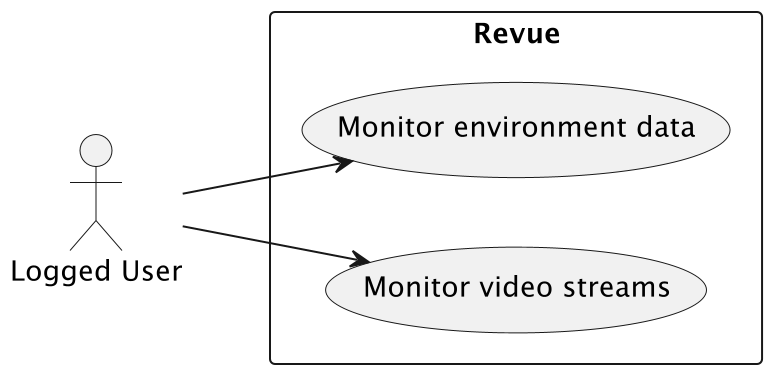
\includegraphics[scale=0.6]{img/simple-use-case}
        \caption{Simple Use Case}
        \label{fig:simple-use-case}
    \end{figure}

    A more complex scenario could involve both sensor and camera usages with the support of a neural network to detect intrusion.
    %
    For example, the director of food wholesale could monitor the temperature of the warehouse and the presence of unauthorized people during the night.
    %
    In this case, the recognition part of the system is necessary to detect whenever an intrusion occurs.

    Moreover, supply chain monitoring can be done for who's needs to ensure that the temperature of
    the warehouse is always in the right range and be alerted whenever the temperature exceeds a certain range to detect or
    prevent problems.

    \begin{figure}
        \centering
        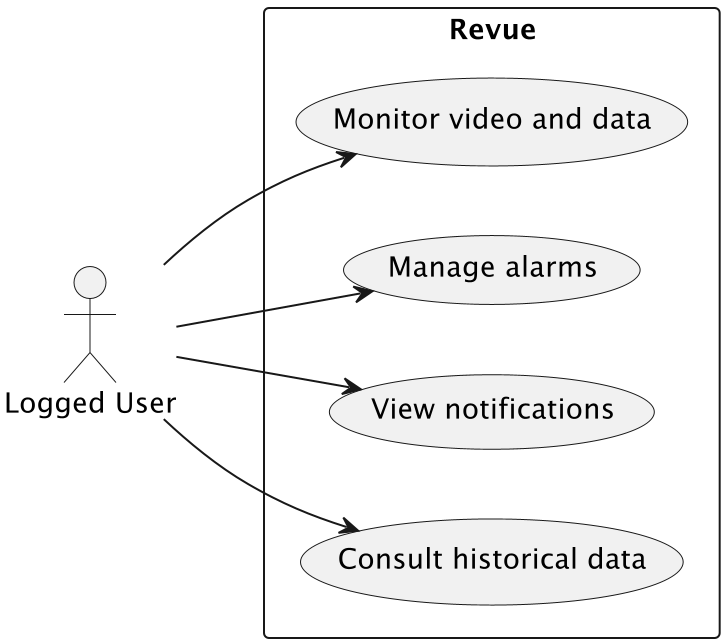
\includegraphics[scale=0.6]{img/advanced-use-case}
        \caption{Advanced Use Case}
        \label{fig:advanced-use-case}
    \end{figure}

    \subsection{Self-assessment policy}

    The project can be considered completed when \textbf{all} requirements are satisfied.

    In particular, non-functional requirements aim to grant a good general quality of the system.
    This will be achieved also using automated tests that will ensure, among other things, the quality of code production.

    \section{Requirements Analysis}

%Is there any implicit requirement hidden within this project's requirements?
%
%Is there any implicit hypothesis hidden within this project's requirements?
%
%Are there any non-functional requirements implied by this project's requirements?

%What model / paradigm / techonology is the best suited to face this project's requirements?
%
%What's the abstraction gap among the available models / paradigms / techonologies and the problem to be solved?

    Drawing up requirements, one relevant considered topic is the recognition feature.
    %
    This is supposed to be developed using Python and exploiting its main libraries for video processing and object recognition, to minimize the abstraction gap.

    Another important aspect is the handling of video streams.
    %
    In fact, to facilitate the development, an implicit requirement is necessary: the use of an ad hoc \textit{media server}.
    %
    This permits also improving the compatibility permitting to produce and consume using different protocols.

    Eventually, internal communications between devices and services need to be guaranteed.
    %
    This implicitly leads to the use of a message broker (\textit{Kafka}) which guarantees better scalability and at least one message delivery policy.


    \section{Design}

    \subsection{Ubiquitous Language}

    For the initial design phase, it's useful to define a common language that permits referring to the concepts with coherence and no ambiguity.
    This is a fundamental part of Domain Driven Design philosophy.

    In \cref{tab:ubiquitous-language} is shown the designed ubiquitous language, while in \cref{tab:synonyms} are reported the synonyms.

    \renewcommand{\arraystretch}{1.5}
    \begin{table}
        \centering
        \begin{tabularx}{0.7\textwidth}{ | c | >{\centering\arraybackslash}X | }
            \hline
            \textbf{Term} & \textbf{Meaning} \\
            \hline
            Camera & Device that records an environment and sends the data to the central system \\
            \hline
            Sensor & Device capturing sensing data from an environment (e.g.\ temperature) \\
            \hline
            Device & Either a camera or a sensor \\
            \hline
            Video Stream & Stream of video data produced by a camera \\
            \hline
            Environment Data & Data produced by a sensor \\
            \hline
            User & User that can access the system \\
            \hline
            Detection & Recognition of an object in a video stream \\
            \hline
            Intrusion & Detection of an unauthorized object \\
            \hline
            Exceeding & Environment value exceeding user defined ranges \\
            \hline
            Anomaly & Either an intrusion or an exceeding \\
            \hline
            Security Rule & Rule defined by the supervisor to trigger anomalies \\
            \hline
            Notification & An alert sent to the user to inform that an anomaly has been triggered. \\
            \hline
        \end{tabularx}
        \caption{Ubiquitous Language}
        \label{tab:ubiquitous-language}
    \end{table}

    \renewcommand{\arraystretch}{1.8}
    \begin{table}
        \centering
        \begin{tabularx}{0.6\textwidth}{ | >{\centering\arraybackslash}X | >{\centering\arraybackslash}X | }
            \hline
            \textbf{Term} & \textbf{Synonyms} \\
            \hline
            Camera & Video camera \\
            \hline
            Video Stream & Video, Transmission \\
            \hline
            Environment Data & Data, Sensing Data \\
            \hline
            User & Supervisor, Admin \\
            \hline
            Security Rule & Rule \\
            \hline
        \end{tabularx}
        \caption{Synonyms}
        \label{tab:synonyms}
    \end{table}

    \subsection{Architecture}

    The overall system is designed with microservices architecture.
    %
    This choice helped us to increase modularity, scalability, reliability and fault tolerance.
    %
    The system is composed of the following microservices:

    \begin{itemize}
        \item \textbf{Authentication Service}: responsible for the authentication and access control.
        \item \textbf{Monitoring Service}: responsible for managing devices and environment data.
        \item \textbf{Recognition Service}: responsible for the recognition of objects in the video streams.
        \item \textbf{Alarm Service}: responsible for the management of the security rules and anomalies.
        \item \textbf{Notification Service}: responsible for sending notifications to the user.
        \item \textbf{Log Service}: responsible for the persistent saving of data.
    \end{itemize}

    Each microservice consists of
    \begin{enumerate*}
        \item Web server exposing REST APIs
        \item Database to store its data (except for the \textbf{Recognition Service})
    \end{enumerate*}
    (\cref{fig:microservice}).

    \begin{figure}
        \centering
        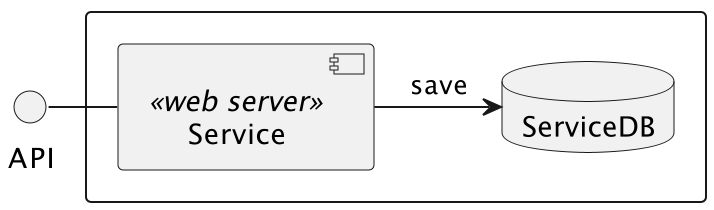
\includegraphics[scale=0.6]{img/microservice}
        \caption{Microservice components}
        \label{fig:microservice}
    \end{figure}

    Moreover, other components are necessary to make the system work:

    \begin{itemize}
        \item \textbf{Frontend}: provides to the user the web interface to interact with the system.
        \item \textbf{Sensors}: capture the environment data and send them to the rest of the system.
        \item \textbf{Cameras}: capture the video streams and send them to the rest of the system.
        \item \textbf{Media Server}: used to consume the produced video streams and make them available using different protocols.
        \item \textbf{Broker}: used to manage some internal communications.
    \end{itemize}

    In \cref{fig:architecture}is presented the whole architecture diagram.

    \begin{figure}
        \centering
        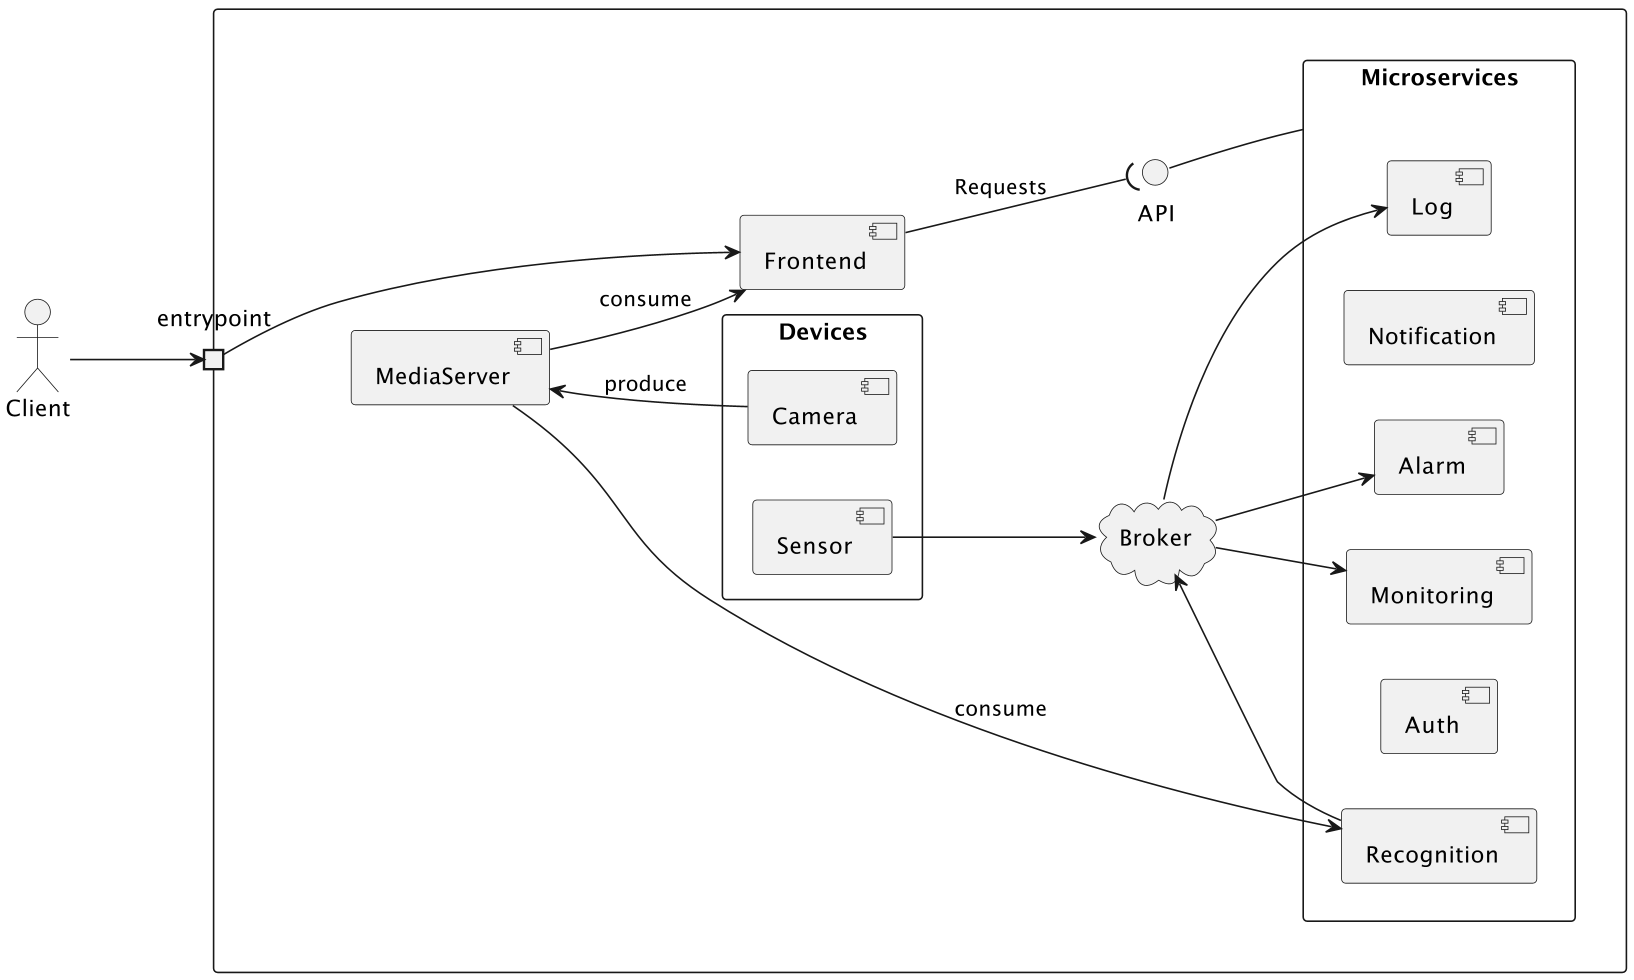
\includegraphics[scale=0.51]{img/architecture}
        \caption{Revue Architecture}
        \label{fig:architecture}
    \end{figure}


    \subsection{Structure}

%    Which entities need to be modelled to solve the problem?
%%
%    (UML Class diagram)
%
%    How should entities be modularised?
%%
%    (UML Component / Package / Deployment Diagrams)

    For the design phase, Domain Driven Design (DDD) and Hexagonal Architecture (HA) have been adopted.
    %
    Actually, the adherence to DDD and HA can be considered a little bit rough (for example, because of the lack of an ad hoc presentation layer) and it will be improved in the future.

    To briefly specify the layers' dependencies:
    \begin{itemize}
        \item \textbf{Domain} layer cannot depend on any other layer.
        \item \textbf{Application} layer (which contains business logic) can depend only on Domain layer.
        \item \textbf{Storage} layer depends on the layers above.
        It is the outer layer since it contains platform-dependent implementation.
    \end{itemize}

    Each microservice has the same structure in terms of classes and packages.
    %
    Furthermore, it is responsible for a specific subset of domain entities.

    In \cref{fig:general-structure}, is represented the general packages/classes structure.

    \begin{figure}
        \centering
        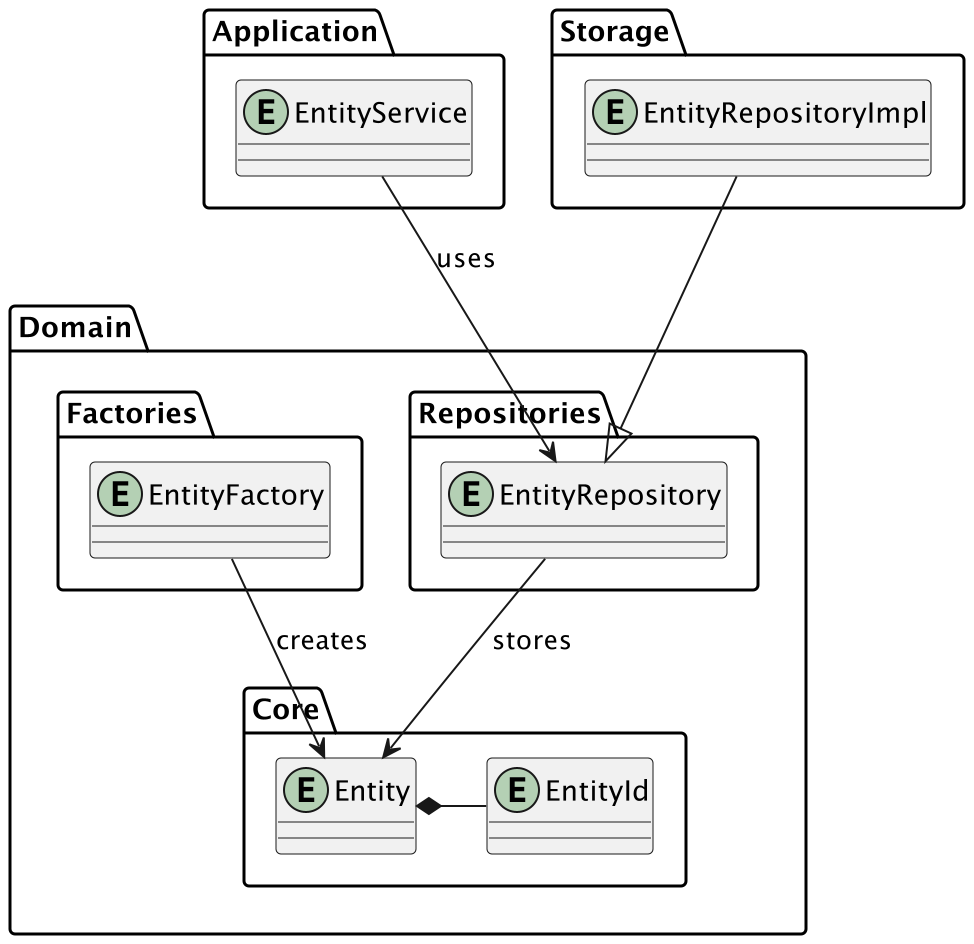
\includegraphics[scale=0.55]{img/general-structure}
        \caption{General structure of microservice}
        \label{fig:general-structure}
    \end{figure}

    \subsection{Behaviour}

    \subsubsection{Monitoring Service}
    \begin{figure}
        \centering
        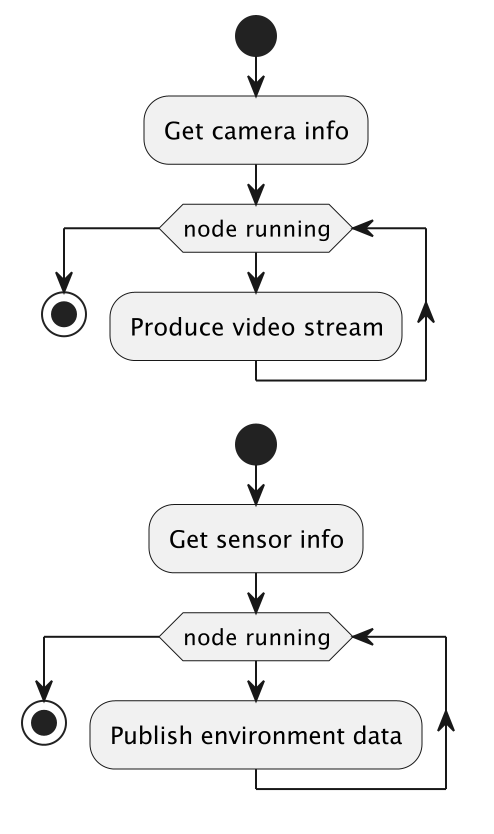
\includegraphics[scale=0.4]{img/device-activity}
        \caption{Device activity diagram}
        \label{fig:device-activity}
    \end{figure}
    Microservice relative to the monitoring of the environment data retrieved from sensors or active streams retrieved from cameras.
    It allows also adding, delete or modify a device configuration, and it is responsible for the management of the devices.

    \subsubsection{Recognition Service}
    \begin{figure}
        \centering
        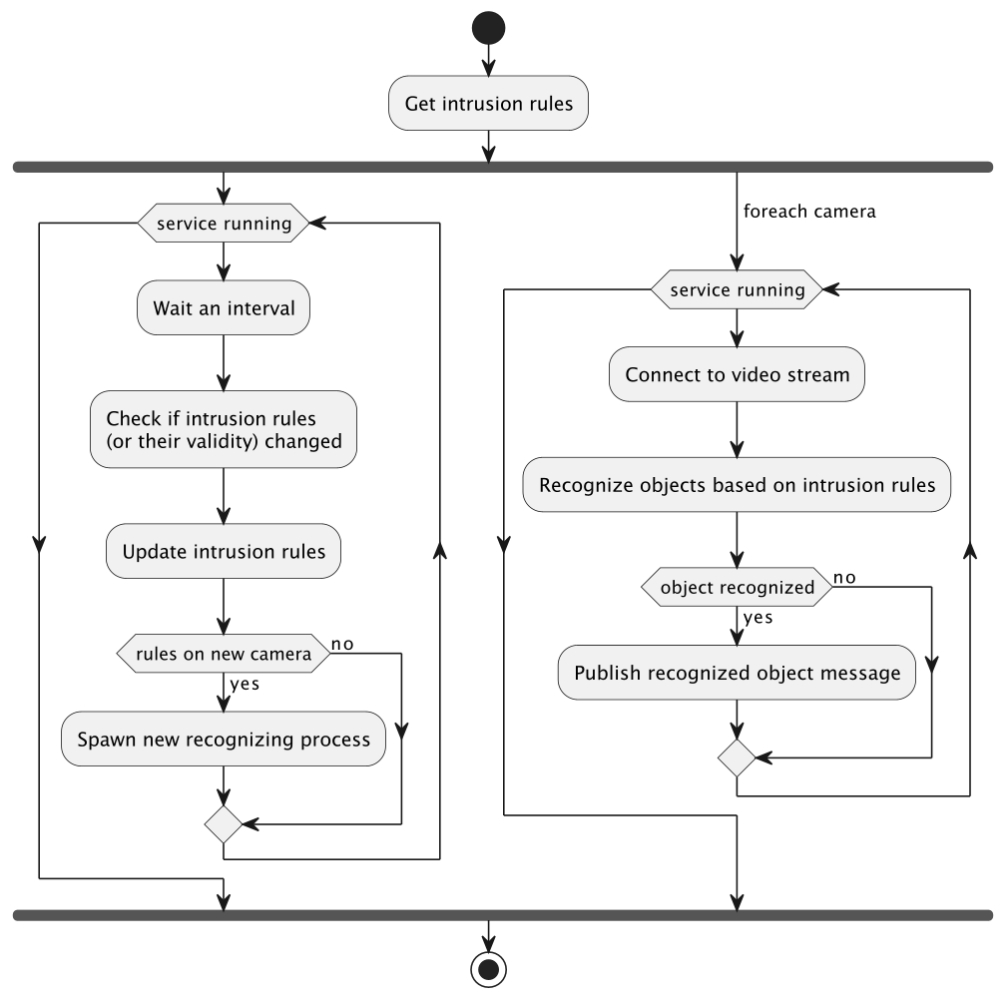
\includegraphics[scale=0.6]{img/recognition-activity}
        \caption{Recognition service activity diagram}
        \label{fig:recognition-activity}
    \end{figure}
    Microservice in charge of object recognition on the camera streams.
    The service is able to recognize a set of predefined objects and notify the Alarm Service, that is in charge of the alarm management.
    For every camera stream, a topic and a recognition process is created and started.
    When a predefined object is recognized it is sent through the relative topic.

    \subsubsection{Alarm Service}
    \begin{figure}
        \centering
        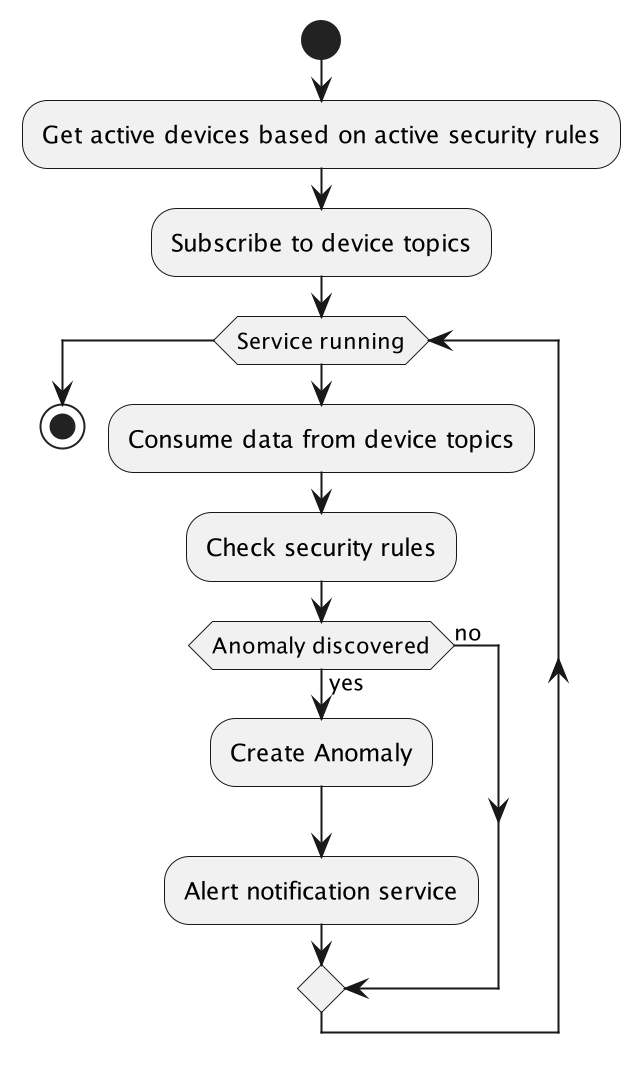
\includegraphics[scale=0.3]{img/alarm-activity}
        \caption{Alarm service activity diagram}
        \label{fig:alarm-activity}
    \end{figure}
    Microservice responsible for the alarm management.
    It is able to check the data coming from the sensors or the recognized objects on cameras' streams.
    The service needs only to check active rules for active devices.
    It is able to create an anomaly, store it and to notify the notification service if the data is not compliant with the rules.
    Moreover, this service is in charge of the management of the security rules, allowing the user to modify their configuration.

    \subsubsection{Notification Service}
    This microservice is responsible to notify the user in case of Anomaly and store them.
    When the Alarm service detects an Intrusion or an Exceeding, it sends a message to the Notification Service that will notify the user.
    Moreover, the notification is in real-time if the user is logged in.

    \subsubsection{Log Service}
    Microservice responsible for the storage of the environment data retrieved from the sensors.
    Moreover, it allows the user to consult the historical data of the environment retrieving them when requested from the persistence.

    \subsection{Interaction}

    \subsubsection{Auth Service}
    \begin{figure}
        \centering
        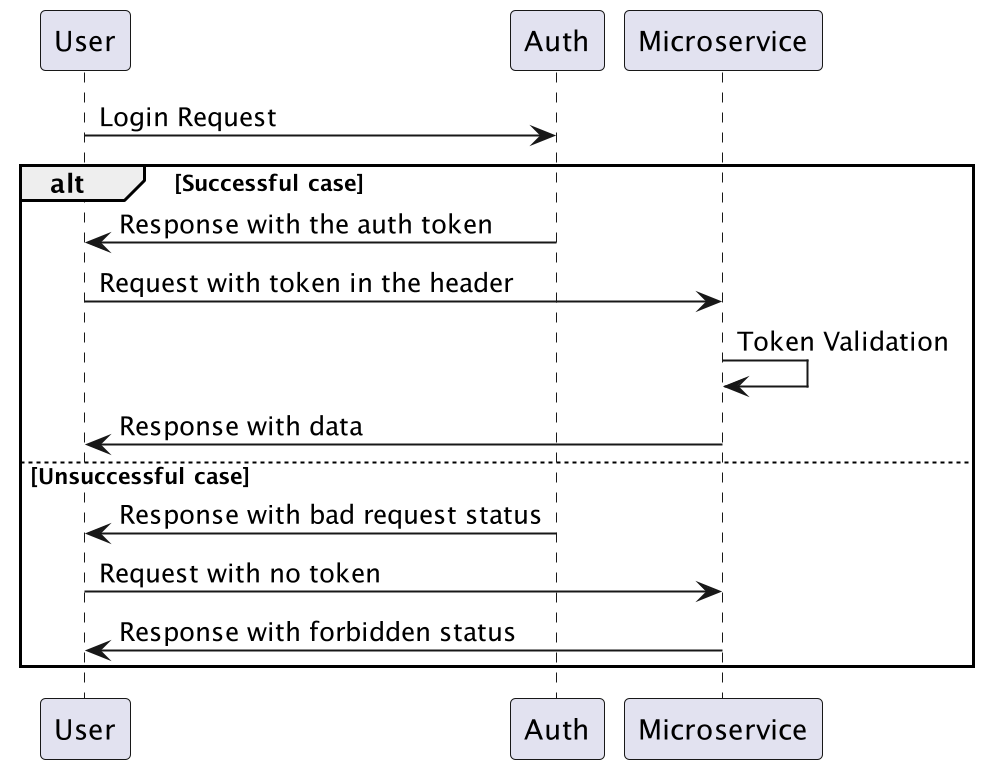
\includegraphics[scale=0.3]{img/auth-service-sequence}
        \caption{Auth service sequence diagram}
        \label{fig:auth-service-sequence}
    \end{figure}
    The Auth Service is responsible for the authentication of the users.
    When a Login request is performed, the Auth Service checks the credentials and returns a token if the user is authenticated.
    When the user wants to perform a request to another service, the user needs only to provide the token in the header of the request.
    Every service contains a validation middleware where the token is checked.
    This process has been implemented through the use of JSON Web Token and sharing the secret key between federated services.

    How should entities interact with each other?
%
    (UML Sequence Diagram)

    \section{Implementation Details}

    \subsection{Kafka}

    \href{https://kafka.apache.org}{Apache Kafka} is the technology chosen to handle intra-system real-time communications.

    In particular, \href{https://kafka.js.org}{KafkaJS} and \href{https://kafka-python.readthedocs.io/en/master/}{kafka-python} clients
    have been used respectively for the \href{https://nodejs.org/en}{Node.js} and \href{https://flask.palletsprojects.com/en/3.0.x/}{Flask} services.

    Kafka is ...

    In the following, is reported the code for producing (\Cref{lst:kafka-producer}) and consuming (\Cref{lst:kafka-consumer}) messages using KafkaJS.

    \lstinputlisting[
        language=TypeScript,
        caption={Producing using KafkaJS},
        label={lst:kafka-producer},
    ]{code/producer.ts}

    \lstinputlisting[
        language=TypeScript,
        caption={Consuming using KafkaJS},
        label={lst:kafka-consumer},
    ]{code/consumer.ts}

    \subsection{Sockets}
    \href{https://socket.io/}{Socket IO} is a library that enables real-time, bidirectional and event-based communication between the browser and the server.
    It has been exploited to implement the real-time communication between the user and the system, in particular for pushing notifications or sending the environment data to the user.
    A security layer has been added to socket servers to ensure secure connections.
    Also for this feature, the JWT token generated when the user logs in has been used.

    \lstinputlisting[
        language=TypeScript,
        caption={Socket Server middleware},
        label={lst:socket-middleware},
    ]{code/sockets.ts}

    \subsection{Object Recognition with YOLO}
    You only look once (\href{https://pjreddie.com/darknet/yolo}{YOLO}) is a state-of-the-art, efficient real-time object detection algorithm.
    %
    YOLO is able to recognize classes of objects and its position in the video.

    This algorithm is used within the \textbf{Recognition} service to perform object recognition on video stream produced by the cameras, according to active security rules.

    In \Cref{lst:object-recognition} is reported the responsible code for this task.
    \lstinputlisting[
        language=Python,
        label={lst:object-recognition},
        caption={Python class performing object recognition with YOLO},
    ]{code/Recognizer.py}


    \subsection{Media Server}
    \href{https://github.com/bluenviron/mediamtx}{MediaMTX} has been used to allow the system to support more than one protocol without implementing a single procedure for each of them.
    All the cameras are linked to the media server, and it can be used to retrieve the streams from the cameras with a single protocol.
    In this case the RTSP protocol has been exploited.

    \subsection{WebRTC}
    To simulate the camera streams, the \href{https://webrtc.org/}{WebRTC} protocol takes place.
    It has been selected for its ability to stream video and audio in real-time with simplicity.
    It does not require any plugin or software installation, it is supported by all the major browsers, and it is open-source.
    Developed by Google, it implements the google congestion control \href{https://www.researchgate.net/publication/316684665_Congestion_Control_for_Real-Time_Communication}{(GCC)} algorithm that allows to stream video and audio in real-time with a low latency.

    \subsection{Single Sign-On}
    \href{https://en.wikipedia.org/wiki/Single_sign-on}{The Single Sign-On (SSO)} has been implemented to allow the user to access the system with a single set of credentials.
    The Auth Service is responsible for the authentication of the user and the generation of the \href{https://jwt.io/}{JWT} token that will be used to authenticate the user in the other services.
    The generated token can be validated from each microservice to ensure that the user is authenticated.
    Following this approach, in case of failure of the authentication service, the user can still access the system until its token validity expires.
    Moreover, the single point of failure is avoided.
    This process has been implemented through the use of \href{https://jwt.io/}{JSON Web Token} and sharing the secret key between federated services.

    \lstinputlisting[
        language=TypeScript,
        caption={Middleware for the microservices},
        label={lst:microservice-middleware},
    ]{code/sso.ts}

    \section{Self-assessment / Validation}

    \subsection{Quality Assurance}\label{subsec:quality-assurance}

    Two main tools have been used to ensure the quality of the code produced:

    \begin{itemize}
        \item \href{https://prettier.io/}{Prettier} is a code formatter that supports many languages.
        It enforces a consistent style by parsing code and re-printing it according to the configuration rules.
        \item \href{https://eslint.org/}{ESLint} Is a tool that statically analyses code to find suboptimal patterns and errors.
    \end{itemize}

    Both tools have been integrated into the Continuous Integration pipeline (\cref{subsec:continuous-integration}) to keep the high-quality code production.

    \subsection{Architectural Testing}\label{subsec:architecture-testing}

    In order to ensure that layers' dependencies are respected, \href{https://github.com/sverweij/dependency-cruiser}{Dependency Cruiser}framework has been exploited.

    Essentially, the configured rules check that:

    \begin{itemize}
        \item \textbf{Domain} layer does not access to any other layer.
        \item \textbf{Application} layer can access only the Domain layer.
        \item \textbf{Presentation} layer can access only Domain and Application layers.
    \end{itemize}

    \subsection{API Testing}\label{subsec:api-testing}

    API testing has been performed using \href{https://vitest.dev/}{Vitest} framework.

    To be able to execute the tests, the database has been mocked using \href{https://github.com/nodkz/mongodb-memory-server}{MongoDB Memory Server}.

    In \Cref{lst:api-test} is reported a simplified example of an API test.

    \lstinputlisting[
        language=TypeScript,
        label={lst:api-test},
        caption={API testing example},
    ]{code/api-test.ts}


    \subsection{Fault Tolerance Testing}\label{subsec:fault-tolerance-testing}

    Since reliability is an important non-functional requirement (requirement\ref{itm:non-func-1}),
    a specific script has been set up to test the system behavior in case of faults.

    In \Cref{lst:fault-tolerance-test} is reported the main part of the script used to
    \begin{enumerate*}
        \item Tearing up the system
        \item Tearing down some running services
        \item Executing fault tolerance tests.
    \end{enumerate*}

    Nevertheless, script and tests could be improved by adding new different fault scenarios.

    \lstinputlisting[
        language=bash,
        label={lst:fault-tolerance-test},
        caption={API testing example},
    ]{code/fault-tolerance-tests.sh}

    \subsection{Continuous Integration}\label{subsec:continuous-integration}

    Each test previously described in this section has been integrated into the Continuous Integration pipeline.



    \section{Deployment Instructions}

    Explain here how to install and launch the produced software artifacts.
%
    Assume the software must be installed in a totally virgin environment.
%
    So, report \textbf{any} configuration step.

    Gradle and Docker may be useful here to ensure the deployment and launch processes to be easy.


    \section{Usage Examples}

    For every usage, the system require a login for security reasons.

    \begin{figure}
        \centering
        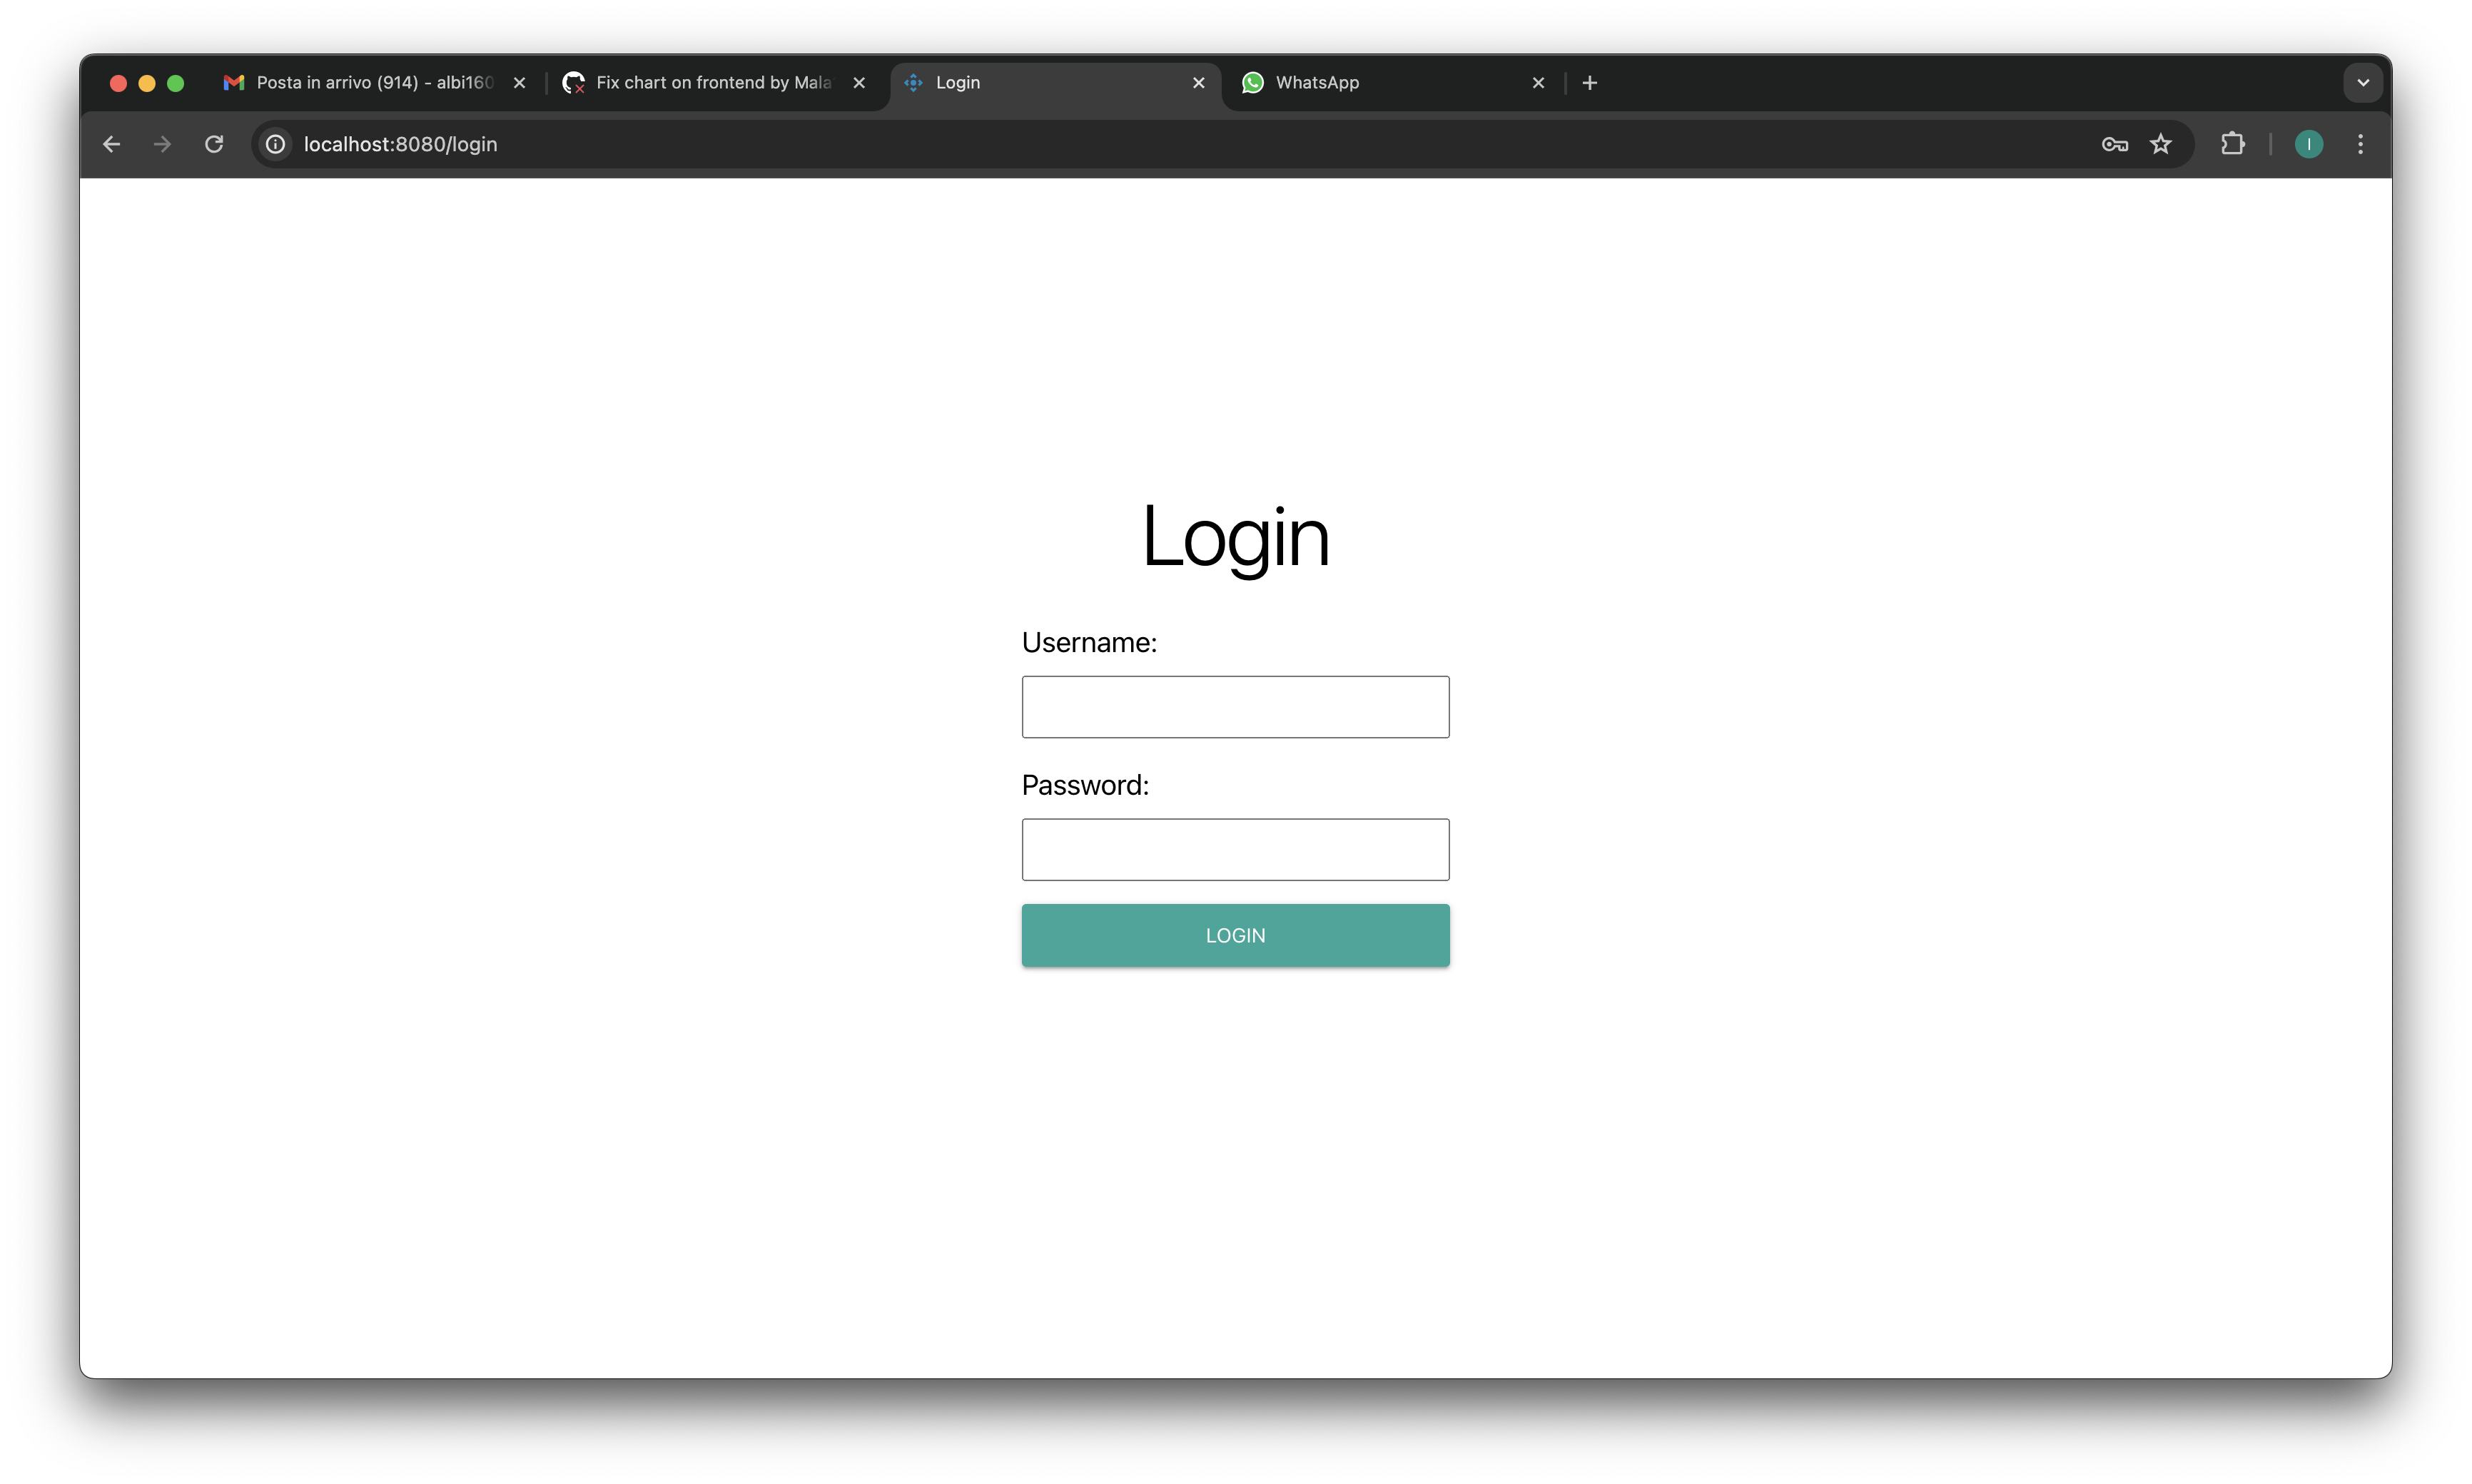
\includegraphics[scale=0.3]{img/usage/login_view}
        \caption{Login view}
        \label{fig:login_view}
    \end{figure}

    In the simplest scenario, the user can see the section designated for sensor environment data or the camera video streams consultation.

    HOME PIC
    \begin{figure}
        \centering
        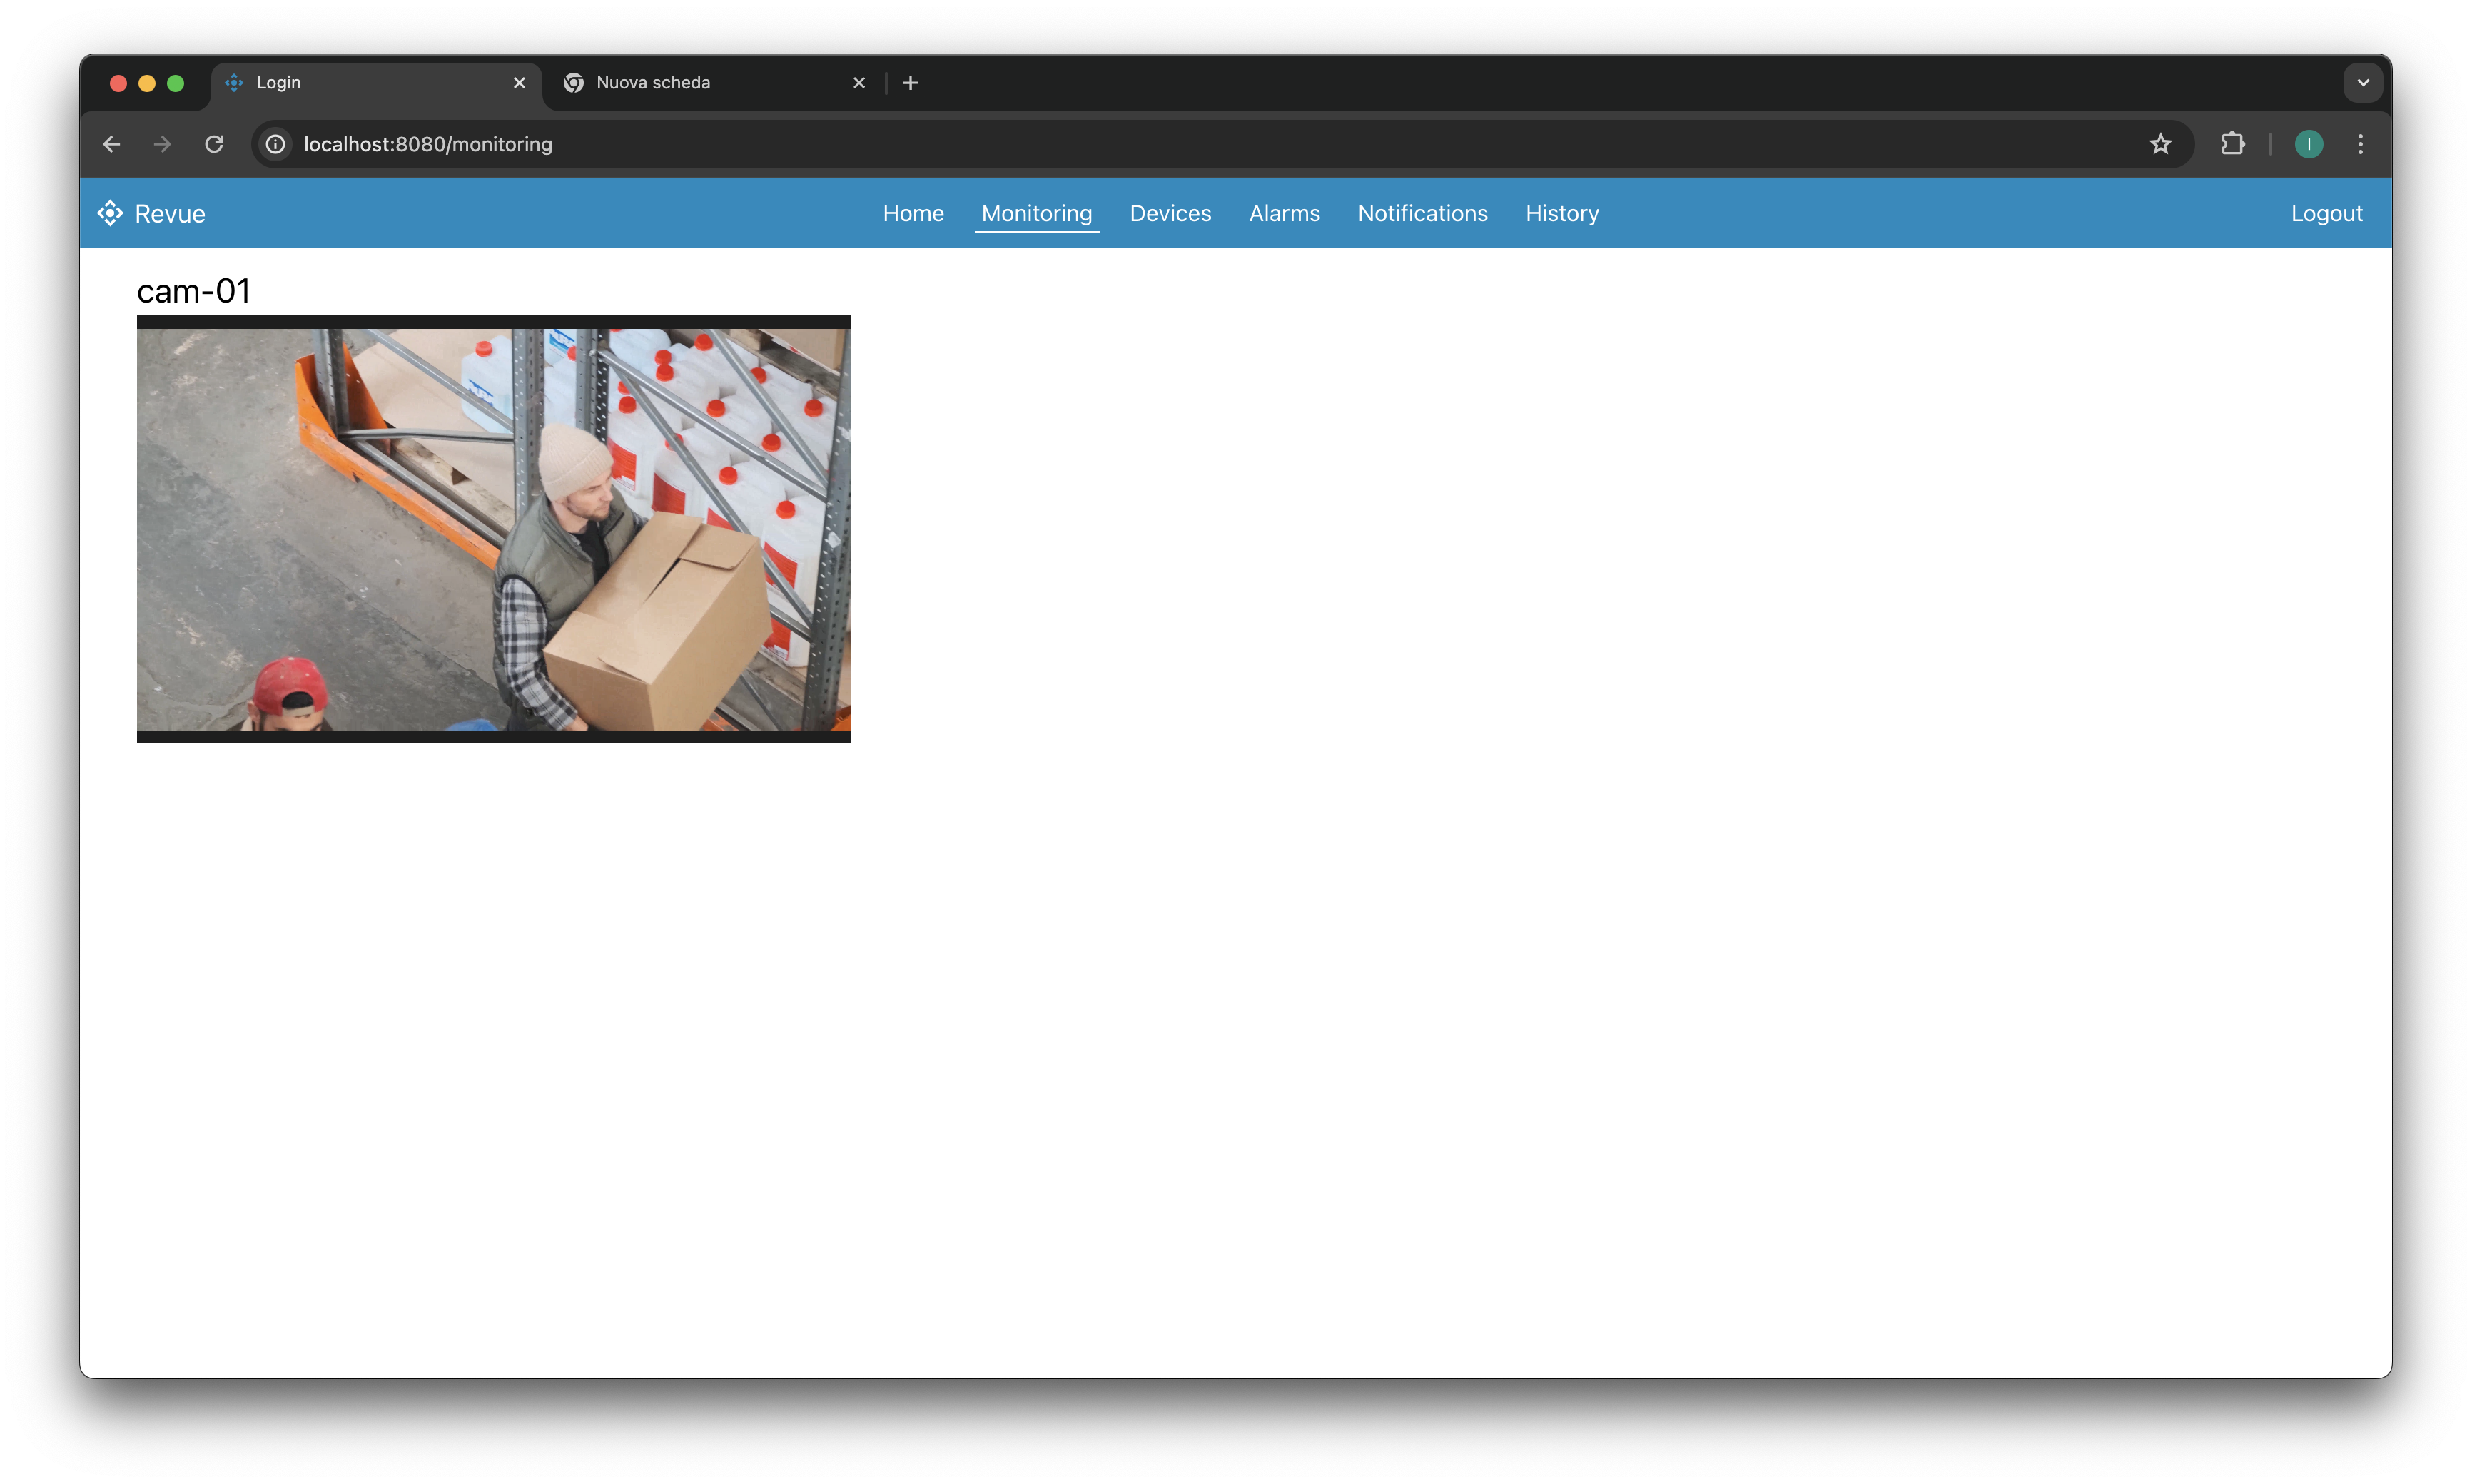
\includegraphics[scale=0.3]{img/usage/camera_view}
        \caption{Monitoring view}
        \label{fig:camera_view}
    \end{figure}


    In the more complex scenario, the user can add security rules to detect exceeding values or unauthorized objects in the video streams.
    When adding a new security rule, the user can choose the object class to detect or the threshold value (for a particular measure) in addition to the device and time slot in which the rule is active.

    \begin{figure}
        \centering
        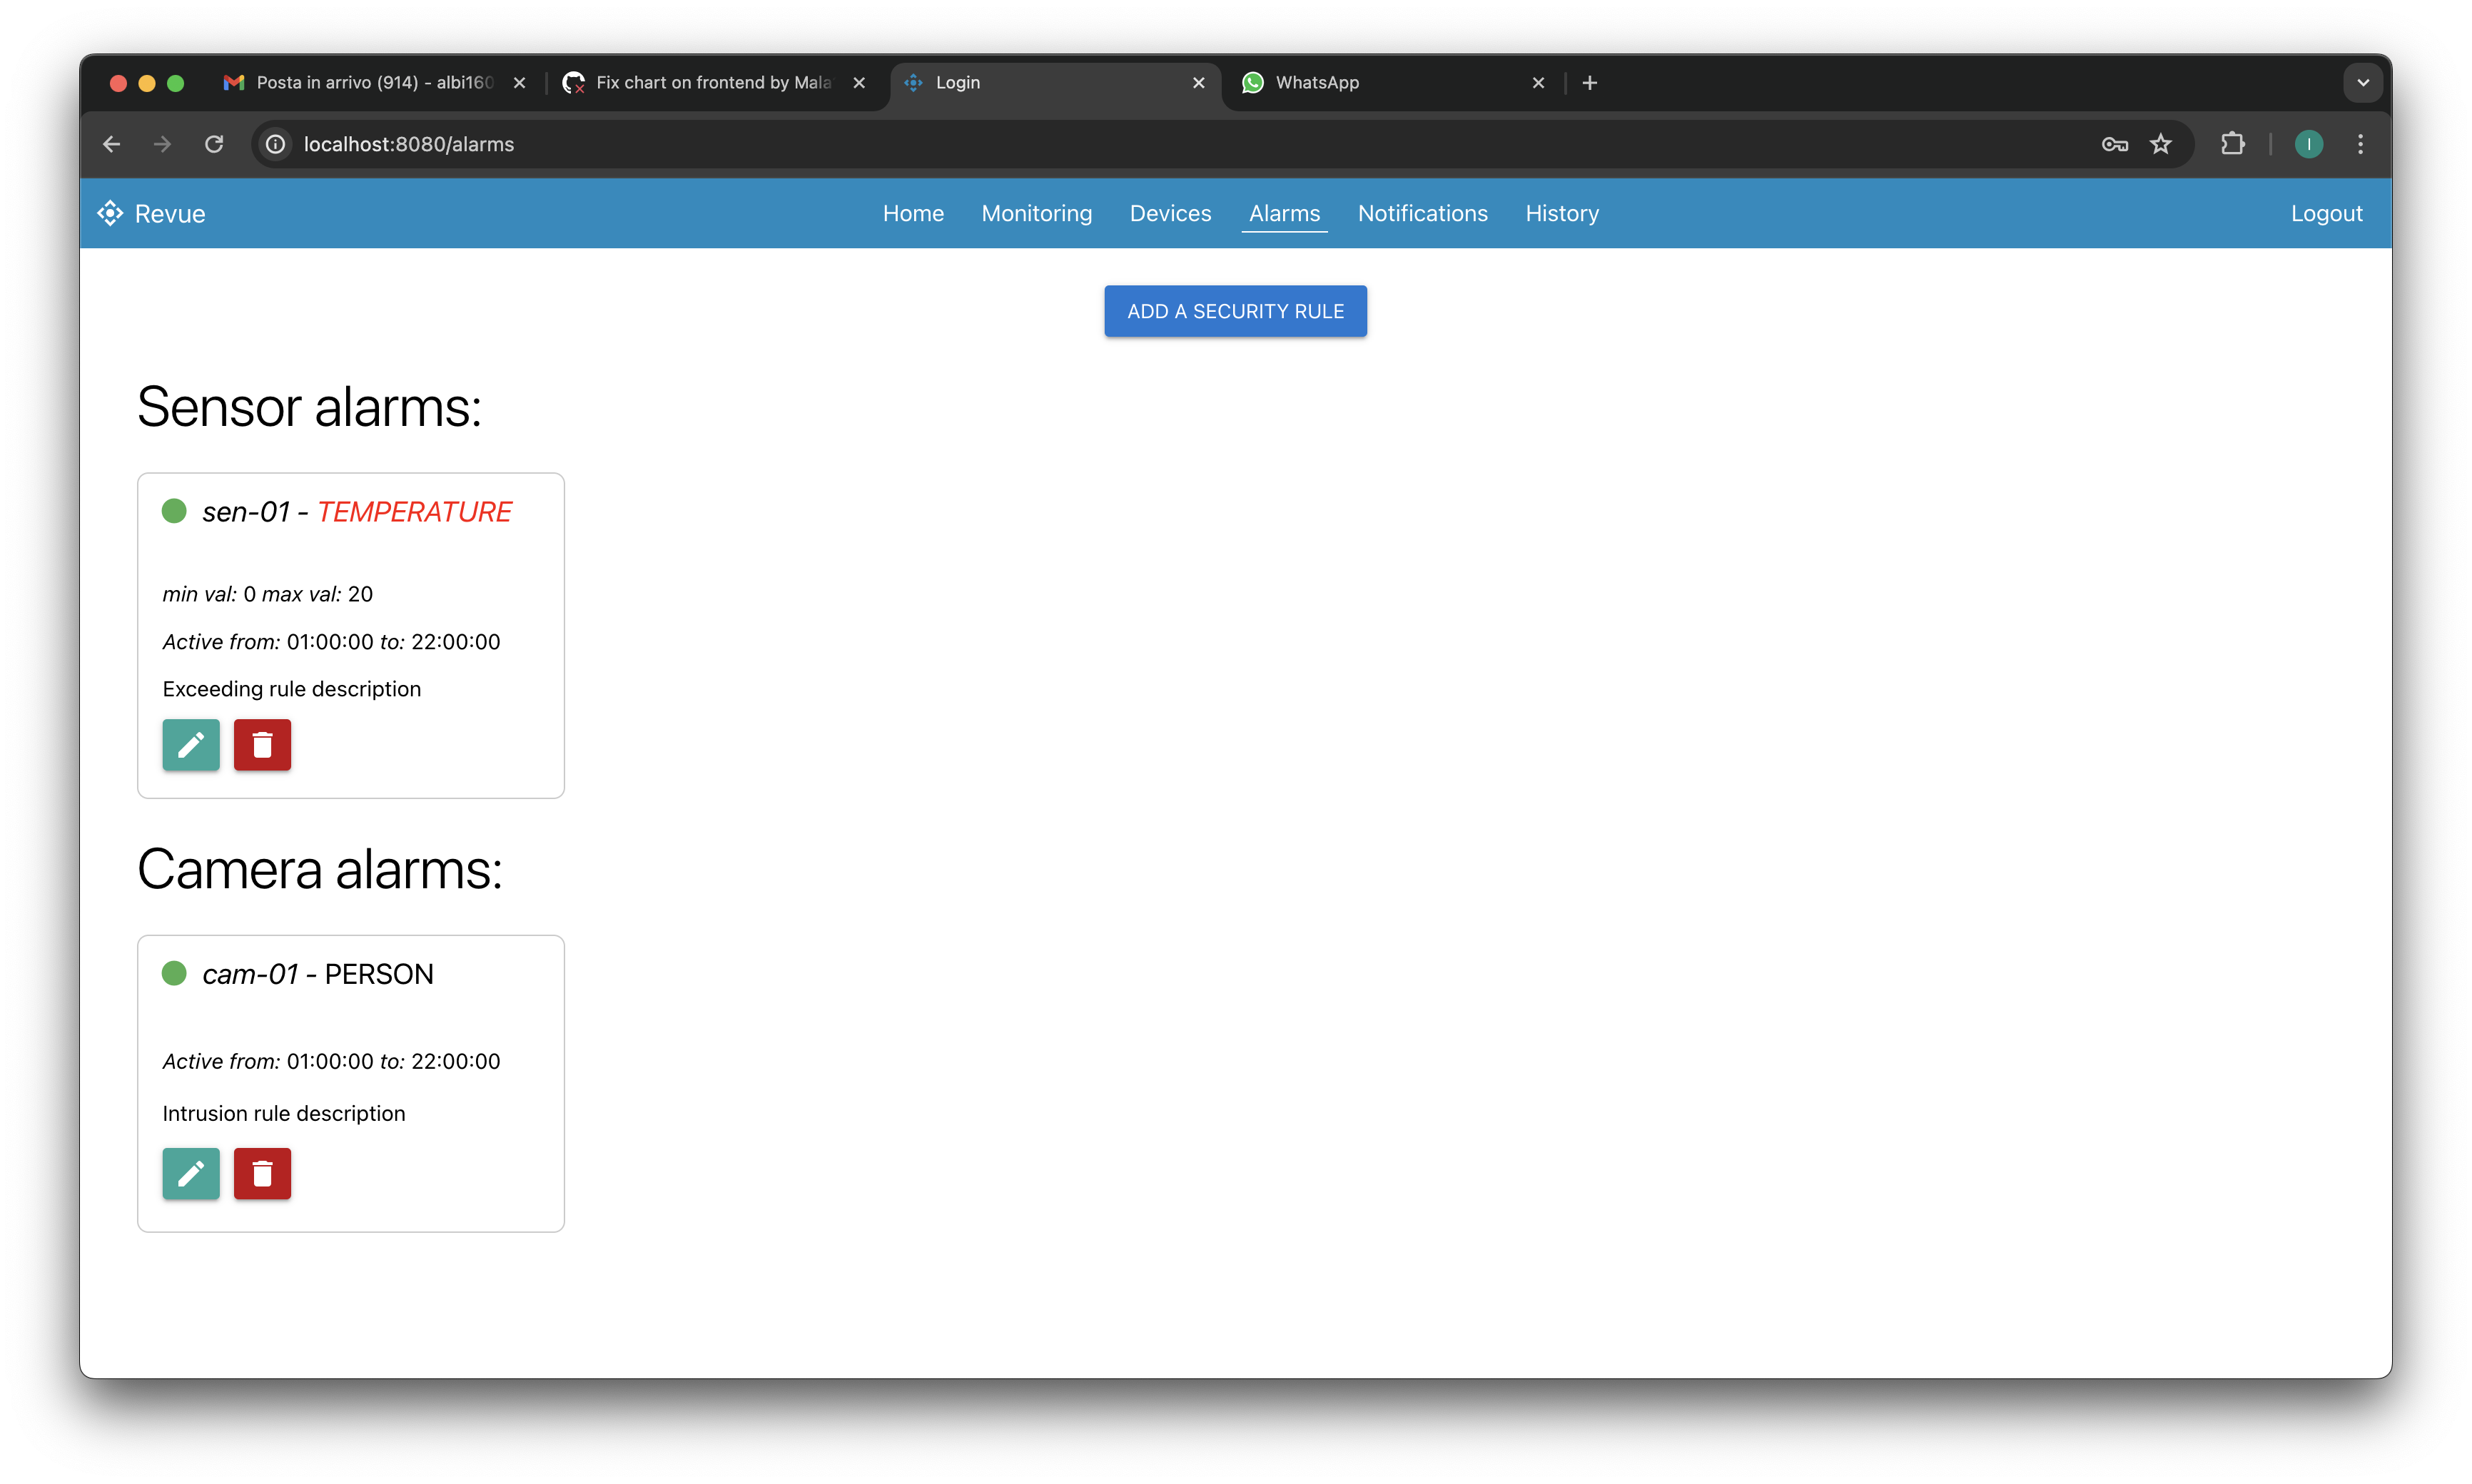
\includegraphics[scale=0.3]{img/usage/security_rule_view}
        \caption{Security rule view}
        \label{fig:security_rule_view}
    \end{figure}

    Both usages of the system consent to the user to add, delete or modify a device or a security rule configuration.

    \begin{figure}
        \centering
        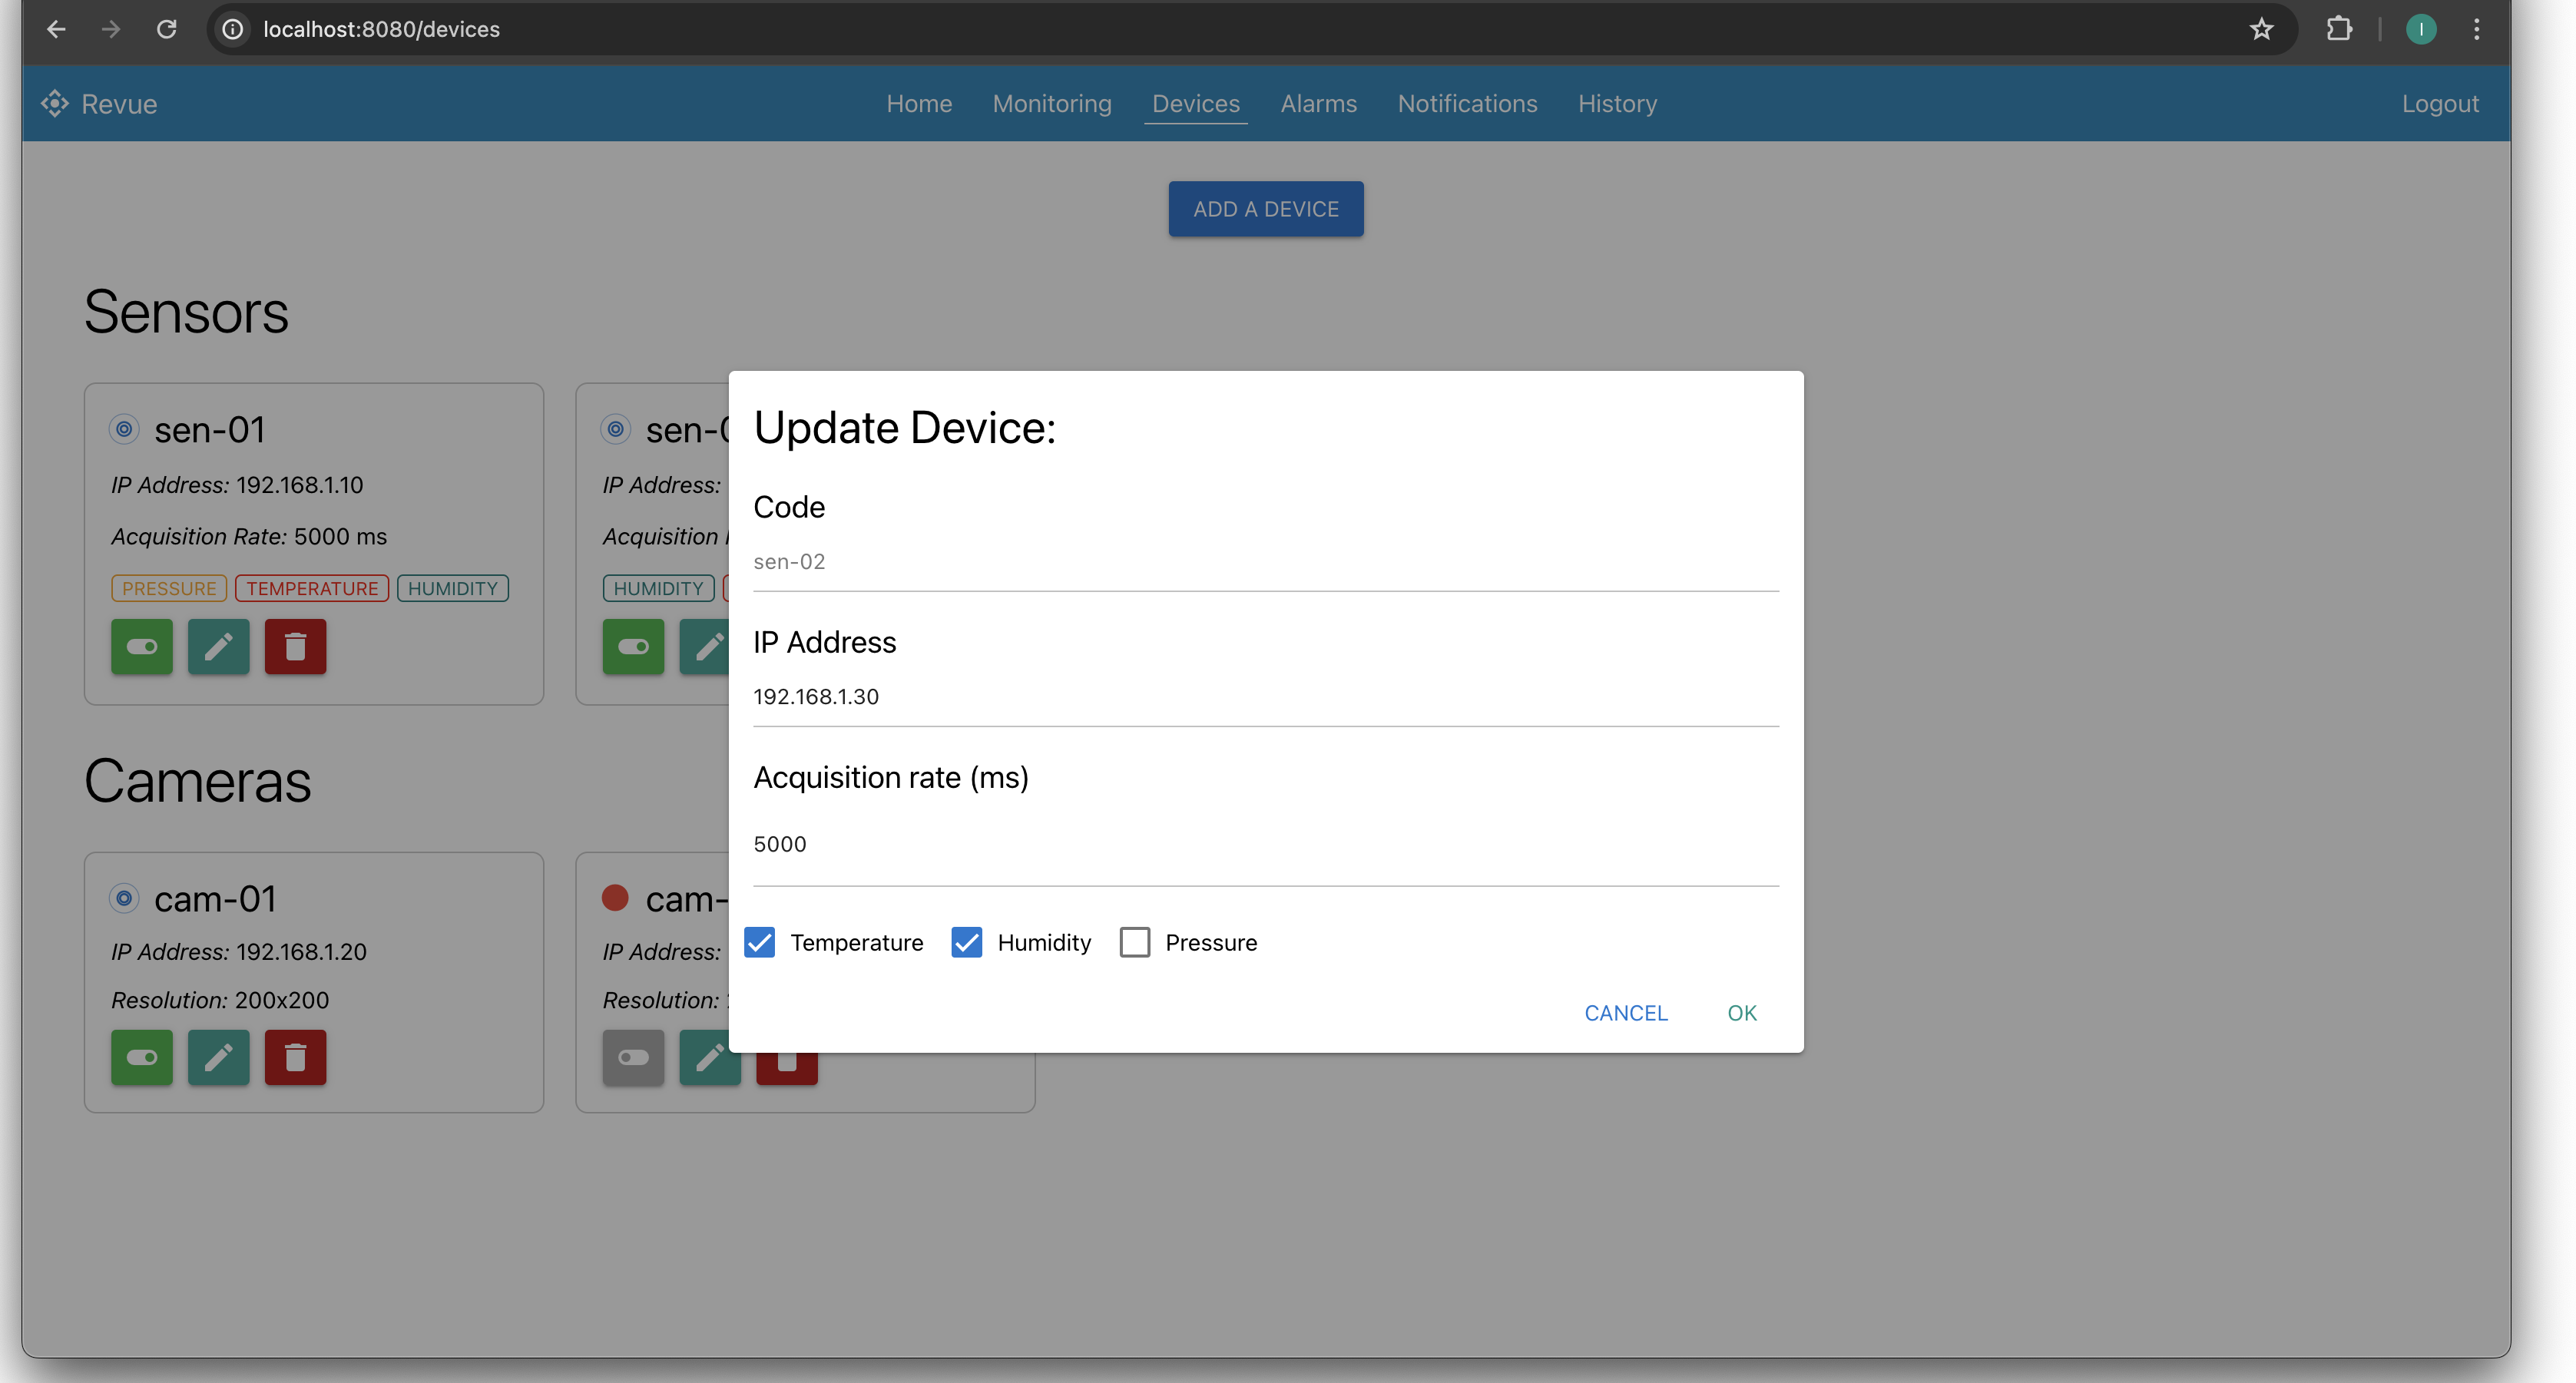
\includegraphics[scale=0.3]{img/usage/update_device_view}
        \caption{Updating a device}
        \label{fig:update_device_view}
    \end{figure}
    \begin{figure}
        \centering
        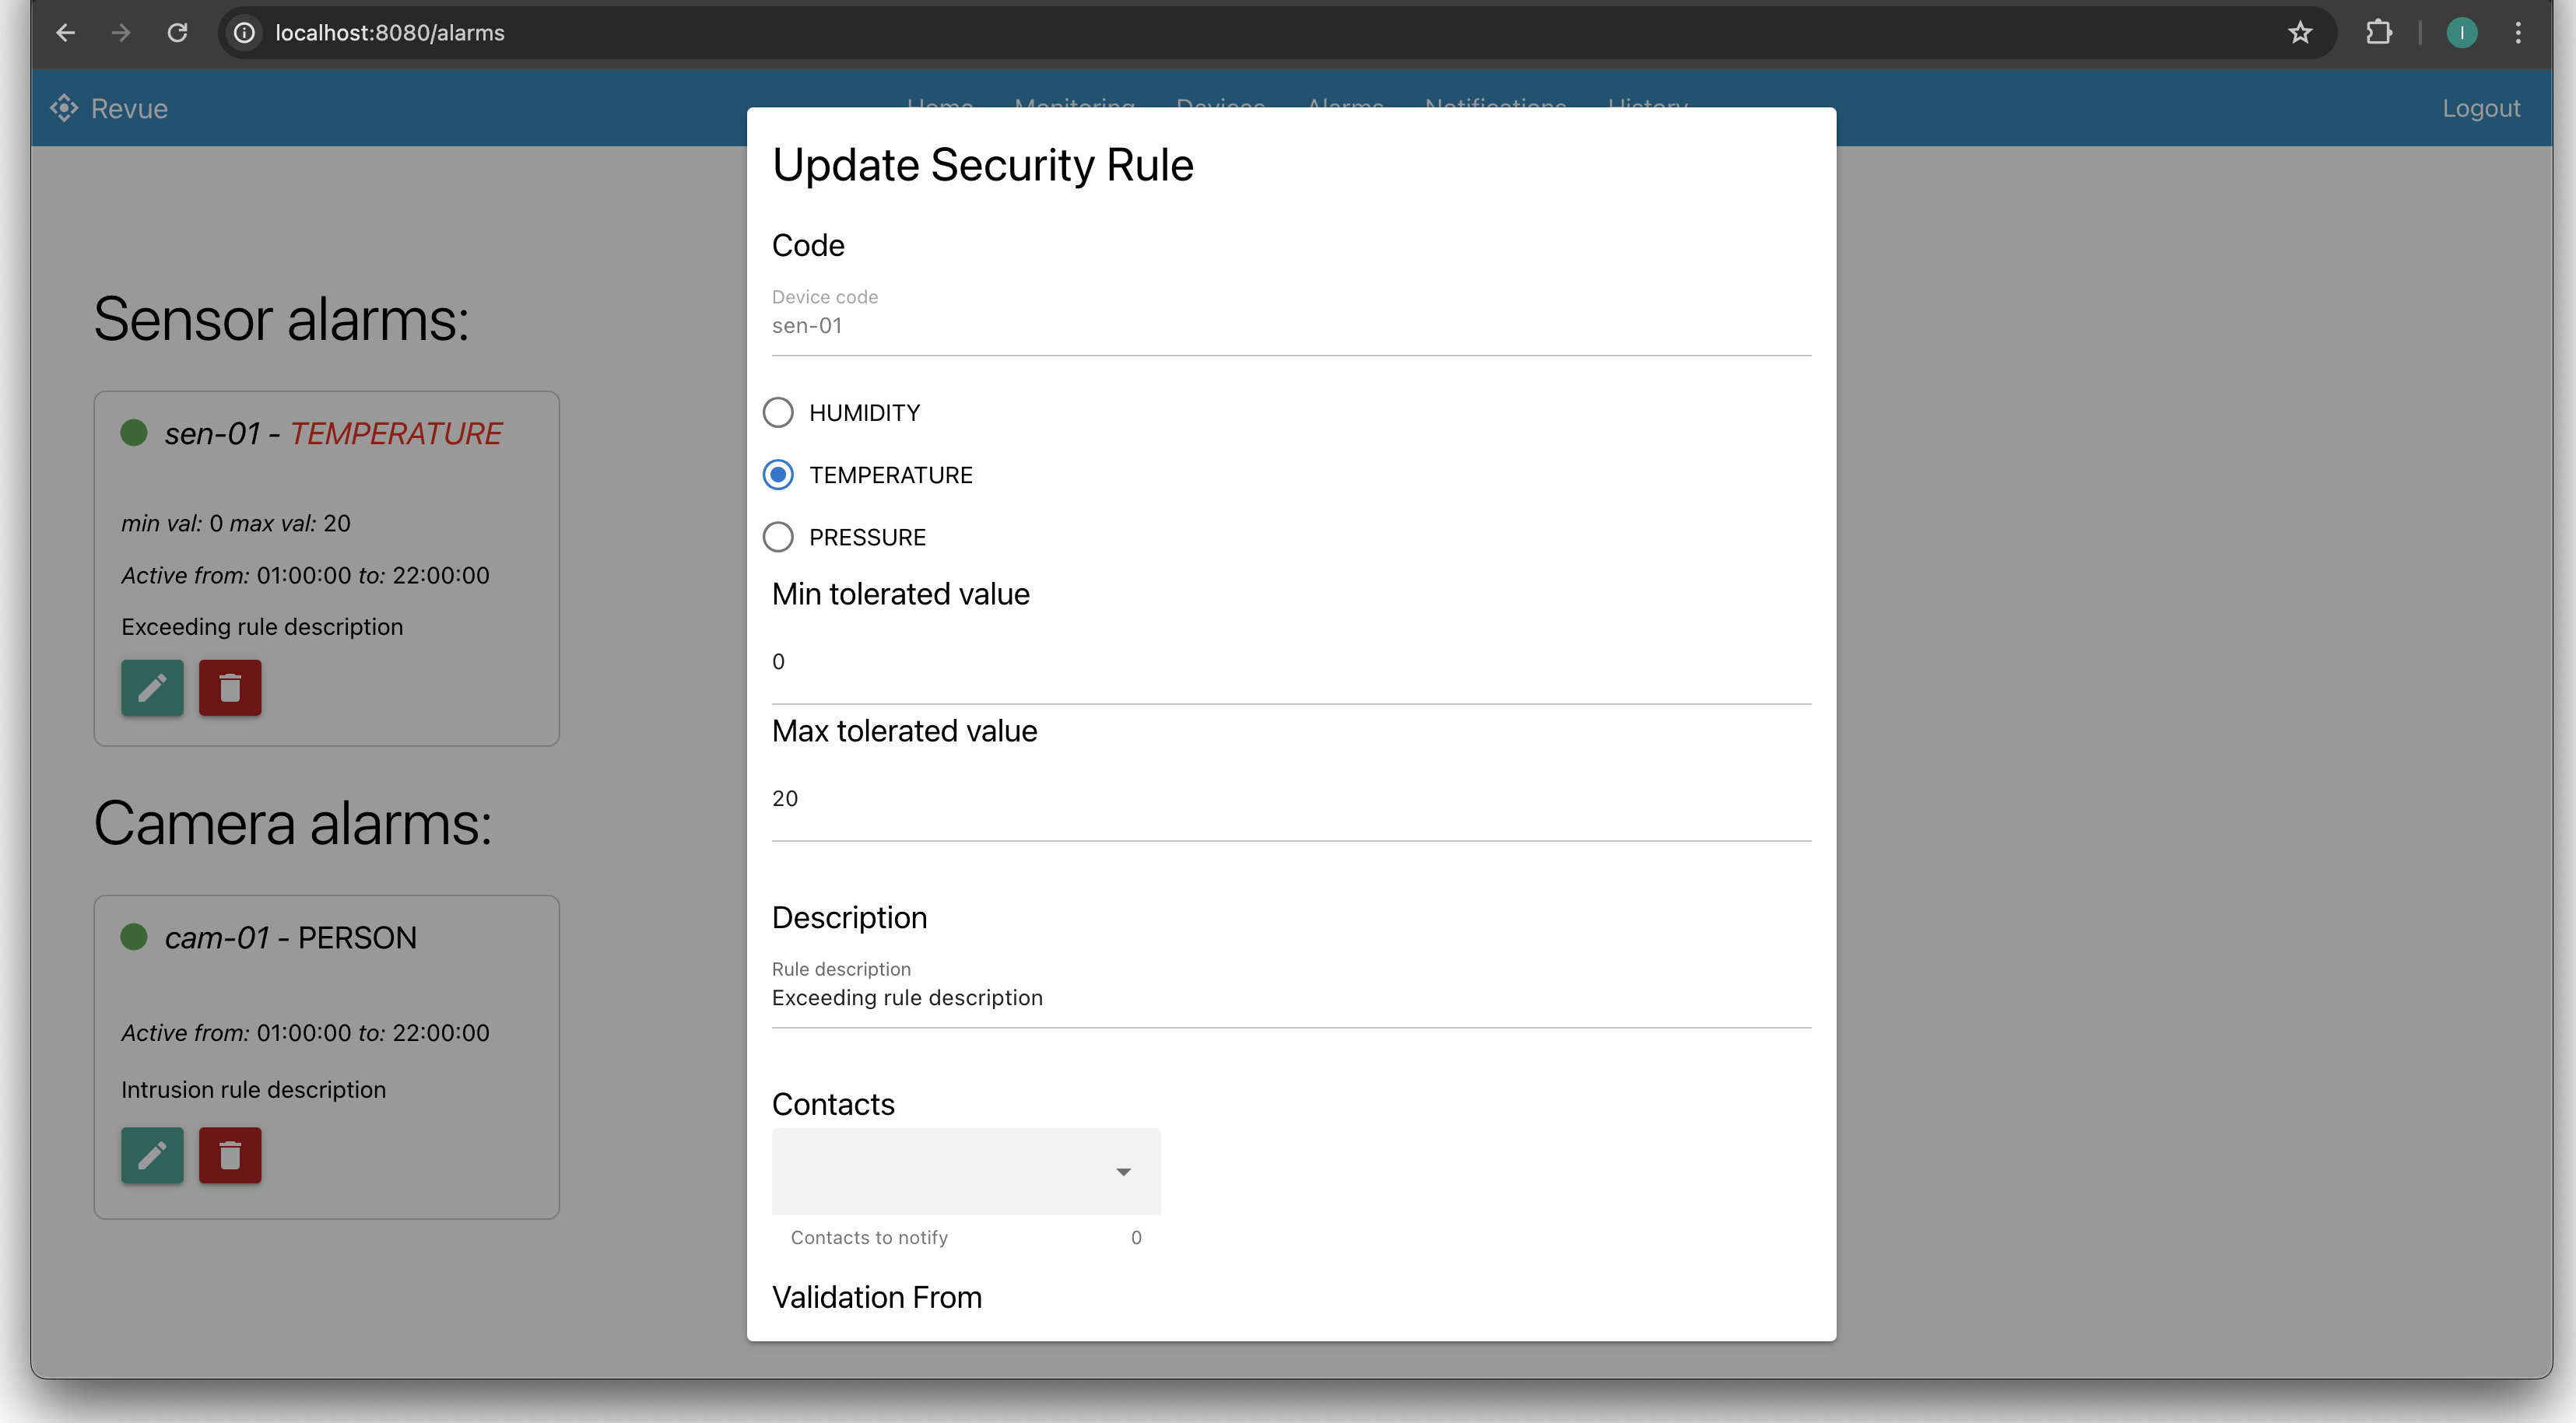
\includegraphics[scale=0.3]{img/usage/update_security_rule_view}
        \caption{Updating a security rule}
        \label{fig:update_security_rule_view}
    \end{figure}

    Moreover, the user can consult the history of produced data or all the notifications received by the system.

    \begin{figure}
        \centering
        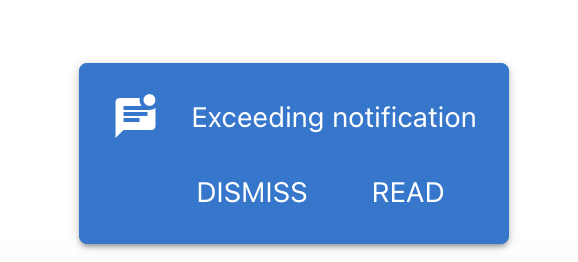
\includegraphics[scale=0.3]{img/usage/notification_example_view}
        \caption{Notification alert}
        \label{fig:notification_example_view}
    \end{figure}
    \begin{figure}
        \centering
        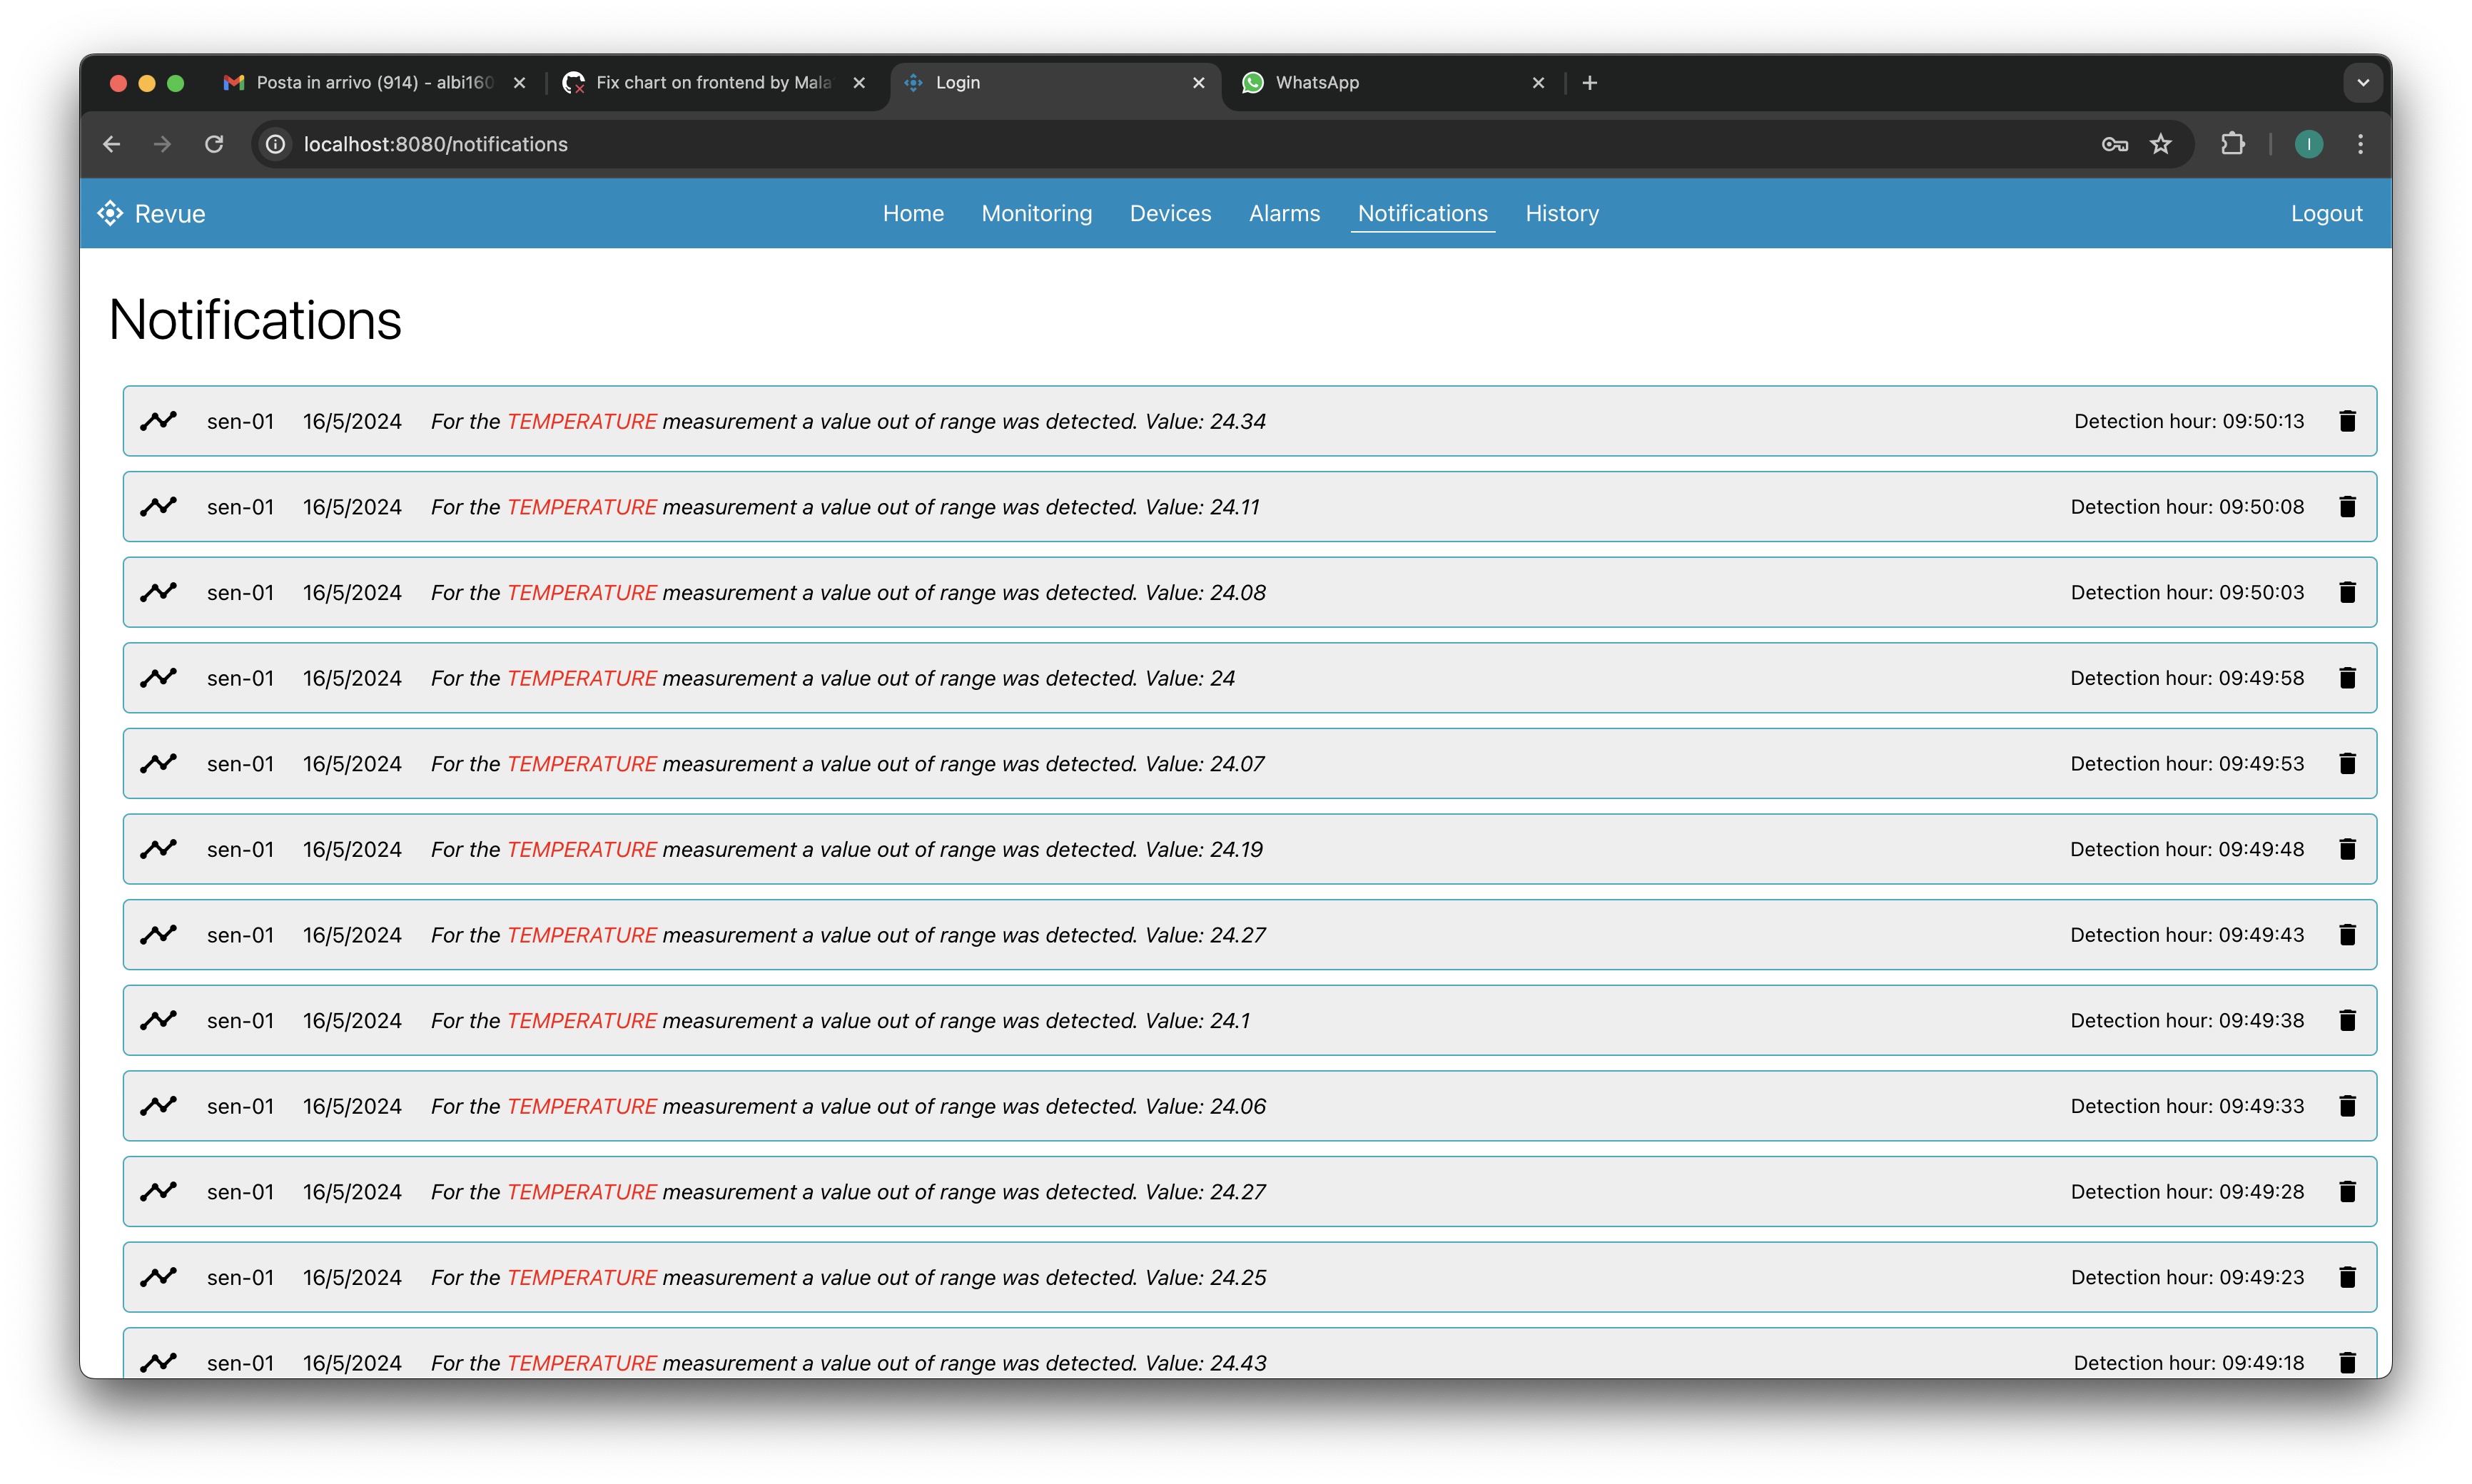
\includegraphics[scale=0.3]{img/usage/notification_view}
        \caption{Security rule view}
        \label{fig:notification_view}
    \end{figure}
    \begin{figure}
        \centering
        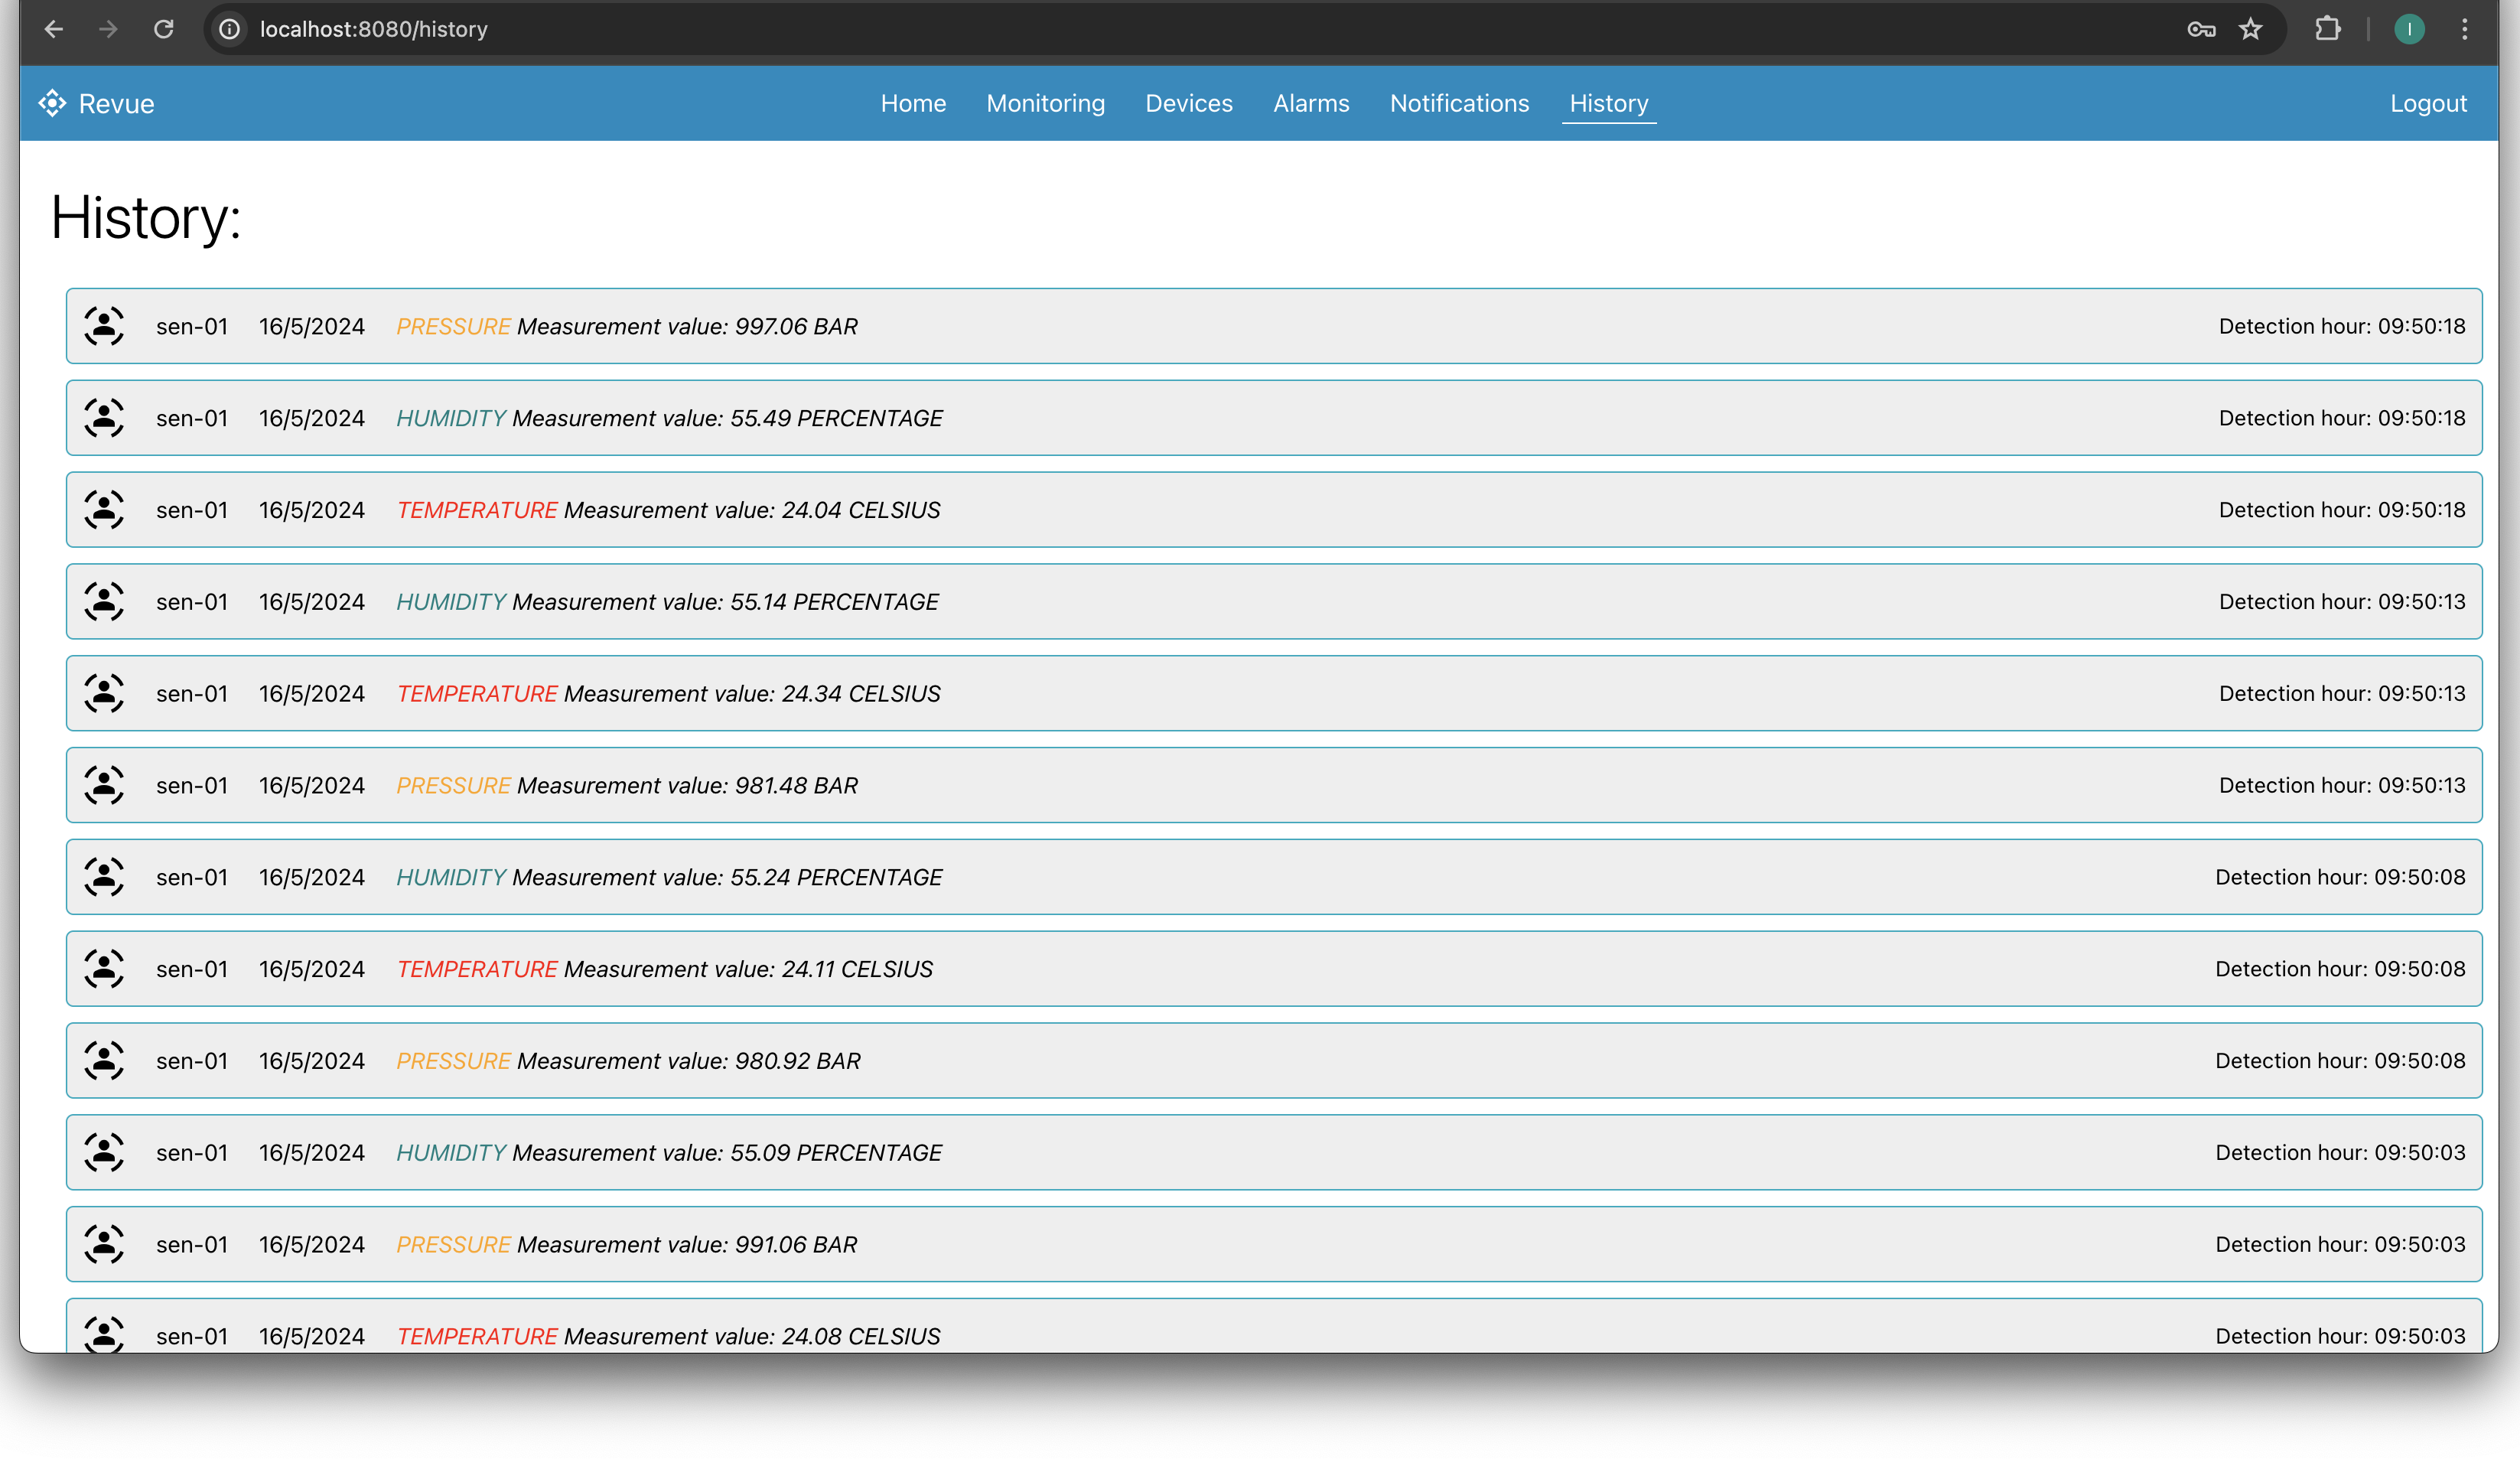
\includegraphics[scale=0.3]{img/usage/log_view}
        \caption{Security rule view}
        \label{fig:log_view}
    \end{figure}


    \section{Conclusions}

    \subsection{Future Works}

    Future developments of this system will certainly have to enrich the user experience to exploit all the possible features offered by the system.
    Certainly a well-designed user section and the introduction of roles could open up to better configurability.

    Real-time video consultation could be improved with the introduction of video recording functions as well as a recorded history,
    which has been put aside for now due to time restrictions.

    Furthermore, Web of Things perspective is the objective for next courses' exams.
    %
    This will lead to the refactor of existent API, the addition of Thing Descriptions, etc.
    %
    Also, an upgrade to the RESTful API could be considered to make them \href{https://en.wikipedia.org/wiki/HATEOAS}{HATEOAS} compliant.

    Another point that could certainly be worked on would be a refinement of the system design to make it even more scalable and maintainable.
    %
    In particular, device management, which is currently part of the monitoring service, surely will be improved with the introduction of a dedicated service.

    For the deployment of the system, the use of Kubernetes (k3s) will be considered to manage the containers in a more efficient way.
    %
    The goal is to deploy the system in a Raspberry PI cluster.

    \subsection{What did we learned}

    This project allowed us to deepen our knowledge of the microservices architecture and to understand the advantages and disadvantages of this approach.

    Moreover, it helped us to experiment with new technologies such as Kafka and a more in-depth testing.

    Fault tolerance testing has been particularly interesting and has allowed us to understand how to manage the system in case of failure of one or more services, validating the reliability of the system.


    \section*{Stylistic Notes}

    Use a uniform style, especially when writing formal stuff: $X$, X, $\mathbf{X}$, $\mathcal{X}$, \texttt{X} are all different symbols possibly referring to different entities.

    This is a very short paragraph.

    This is a longer paragraph (notice the blank line in the code).
    It is composed of several sentences.
%
    You're invited to use comments within \texttt{.tex} source files to separate sentences composing the same paragraph.

    Paragraph should be logically atomic: a subordinate sentence from one paragraph should always refer to another sentence from within the same paragraph.

    The first line of a paragraph is usually indented.
%
    This is intended: it is the way \LaTeX{} lets the reader know a new paragraph is beginning.

    Use the \href{https://en.wikibooks.org/wiki/LaTeX/Source_Code_Listings}{\texttt{listing}} package for inserting scripts into the \LaTeX{} source.

    \nocite{*} % Includes all references from the `references.bib` file
    \bibliographystyle{plain}
    \bibliography{references}

\end{document}
